%chapter 6
\chapter{The MODES Detector and System Integration}

The detector assembly and integration of the whole system is a formidable task. Spanning from the design phase to the full installation phase of the project, all phases are presented in this chapter.  

\section{System Requirements}
There are four main requirements imposed on the system and are fundamental to the system integration design. These are:
\begin{itemize}

	\item \textbf{Modularity} - The system must allow for users to move and mount the detector array in any desired fashion. This requires that the system can be broken down to several key modules that form the base of the system. In order to be assembled by a single user then imposes a weight restriction on each module of 25 kg.
	\item \textbf{Portability} - The system must be portable. The ability to relocate and operate is absolutely necessary and the assembled system must be able to probe while in motion.
	\item \textbf{Durability} - The system must be able to operate for extended periods of time without failure. Due to the other requirements this is very important as the system must be able to withstand being disassembled and relocated.
	\item \textbf{Safety} - The system must be safe to assemble and operate for all users, including non-experts. Measures must be introduced to reduce the risk of accidents and provide maximum protection in case such events occur.
\end{itemize}

\section{The Detectors}
The prototype consists of 8 fast neutron, 2 thermal neutron and 2 gamma detectors. The detectors are of cylindrical design with an extrusion in the form of the valve. The fast neutron detector tube is 1000 mm in length and has a diameter of 70 mm at the widest part, shown in figure \ref{fig:fastNeutronDetectorDims}. With the inclusion of the valve gives a height of 200 mm. The thermal neutron detectors match these dimensions and only differ by having a $^{6}$LiF coating internally. Each neutron detector tube is composed of steel and has a total weight of 5.0 kg. 

\begin{figure}[htbp]
\begin{center}
\includegraphics[width=120mm]{Chapter6/figures/fastNeutronDetector.png}
\caption{The dimensions of the fast and thermal neutron detectors.}
\label{fig:fastNeutronDetectorDims}
\end{center}
\end{figure}

The gamma detectors are larger in diameter, at 140 mm, but shorter in length, at 607 mm, and with the inclusion of the valve the height is 290 mm. This is shown in figure \ref{fig:gammaDetectorDims}. They are considerably heavier than the neutron detectors at approximately 11 kg. The gamma detector vessel is made from Titanium.

\begin{figure}[htbp]
\begin{center}
\includegraphics[width=140mm]{Chapter6/figures/gammaDetector.png}
\caption{The dimensions of the gamma detectors.}
\label{fig:gammaDetectorDims}
\end{center}
\end{figure}

In order to satisfy the system requirements these detectors must be housed in appropriate containers. It is obvious that this cannot be done with one container alone, as this would exceed the 25 kg limit without taking into account the weight of the container itself. Therefore the choice of the container skin, and hence the material, is crucial in the design of the detector casing.

\section{Detector Container Design}
Rectangular boxes are implemented for the container designs, this makes them easily configurable and can then be stacked upon each other. The neutron detectors are paired and housed in containers of external dimensions 1255 $\times$ 170 $\times$ 250 mm, shown in figure \ref{fig:neutronDetectorContainer}. Due to the larger dimensions and weight of the gamma detectors these are housed individually in boxes of external dimensions 1005 $\times$ 170 $\times$ 300 mm, shown in figure \ref{fig:gammaDetectorContainer}.

\begin{figure}[htbp]
\begin{center}
\includegraphics[width=140mm]{Chapter6/figures/neutronDetectorBoxGraphic.png}
\caption{The dimensions of the neutron detector container. All dimensions are shown in mm.}
\label{fig:neutronDetectorContainer}
\end{center}
\end{figure}

\begin{figure}[htbp]
\begin{center}
\includegraphics[width=140mm]{Chapter6/figures/gammaDetectorBoxGraphic.png}
\caption{The dimensions of the gamma detector container. All dimensions are shown in mm.}
\label{fig:gammaDetectorContainer}
\end{center}
\end{figure}
  
\section{Detector Container Material}
A suitable detector container material must be lightweight while maintaining structural support and protection for the detectors. Radiation shielding is also a key factor when deciding on the material and heavy consideration must be focused on minimising this effect. 

Carbon fiber is a seemingly perfect candidate for the detector material, as it is renowned for its high tensile strength while maintaining a very low density. However it is expensive to produce and would not provide shielding from ElectroMagnetic (EM) noise. This could be overcome by adding a layer of conductive material but it would prove difficult to manufacture for a casing design. Plastics, such as polyethylene and polypropylene, are very light but are also soft and would not provide enough structural support. In order to provide EM shielding as well, metals are the primary candidate, with a composition of metals and materials favourable. The materials considered are shown in the table \ref{tab:casingMaterials}.

\begin{table}[!htbp]
\begin{center}
	\begin{tabular}{l*{4}{c}r}
	\hline
	 \hline
	 Material & Composition & Density & Youngs Modulus & Electrical Conductivity \\
    	\hline
   	- & - & gcm$^{-3}$ & GPa & Sm$^{-1}$ \\
    	\hline
    	Carbon fiber & C$_{3}$H$_{3}$N & 1.4-1.8 & $\sim$50-100 & - \\
    	Polyethylene & C$_{2}$H$_{4}$ & 0.9 & $\sim$0.1-2 & - \\
    	Polypropylene & CH$_{2}$=CHCH$_{3}$ & 0.9 & $\sim$1.5-2 & - \\
    	Aluminium & Al & 2.7 & $\sim$69 &  3.5$\times$10$^{7}$ \\
    	Magnesium & Mg & 1.7 & $\sim$45 &  2.2$\times$10$^{7}$ \\
    	Iron & Fe & 7.87 & $\sim$200 &  1.0$\times$10$^{7}$\\
    	Lead & Pb & 11.35 & $\sim$16 &  4.9$\times$10$^{6}$ \\
    	\hline
    	\hline
  	\end{tabular}
	\caption{Summary of potential materials considered for the casing.}
    	\label{tab:casingMaterials}
\end{center}
\end{table}

Of the metals shown, aluminium is the most ideal candidate due to its reasonably low density, relative strength and high conductivity. Iron and lead are far too dense to be considered and have lower conductivities, whereas magnesium is less dense but is brittle and is susceptible to corrosion. Compared to carbon fiber aluminium is rather dense at 2.7 gcm$^{-3}$, which will severely impede on the weight restrictions. To reduce the weight, a honeycomb aluminium structure is considered. The effect is significant on the weight as the equivalent density of the honeycomb layer is 0.29 gcm$^{-3}$. The honeycomb structure is of 5.2 mm thickness and is then sandwiched between two thin aluminium sheets, each of 0.5 mm, to maintain the structural support. The casing material is shown in figure \ref{fig:casingMaterialGraphic}.

\begin{figure}[htbp]
\begin{center}
\includegraphics[width=100mm]{Chapter6/figures/casingMaterialGraphic.png}
\caption{The honeycomb aluminium structure used for the containers skin.}
\label{fig:casingMaterialGraphic}
\end{center}
\end{figure}

\subsection{Monte Carlo Studies}
Monte Carlo (MC) simulations are implemented to gain an understanding of the effects such a casing would introduce to the incident energy spectra of neutrons and gammas. Geant4 \cite{GEANT} is used to study particle interactions within the casing and record information on these for large amounts of events. A hypothetical source of neutrons and gammas with a flat and isotropic kinetic energy spectrum is implemented in the simulation. With energies ranging from 50 keV to 15 MeV the energy regime of interest for the MODES-SNM project can be probed. The source is implemented at a distance of 0.5 m from the casing with source dimensions of 1 $\times$ 1 $\times$ 1 cm$^{3}$. One layer of the casing is modelled as a solid sheet of 1.0 mm thick aluminium (100\% $^{27}_{13}$Al), density 2.7 gcm$^{-3}$, on top of a sheet of the same aluminium composition but with 5.2 mm thickness and a lower density of 0.29 gcm$^{-3}$. This casing plate then has dimensions of 1000 mm $\times$ 1000 mm $\times$ 6.2 mm, shown on the left of figure~\ref{fig:casingDiagram}. The source and casing plate are situated in a vacuum with the complete experimental setup shown on the right of figure~\ref{fig:casingDiagram}. 

Only information on the primary particle is of interest for this study and tracking is setup to propagate the primary until it is either outside the main experimental boundaries or it is absorbed. The particles kinetic energy, momentum and position are recorded upon reaching the casing and once more upon leaving the casing. All primaries are recorded that pass through the casing boundary, regardless if energy is deposited or not. 1 $\times$ 10$^{6}$ primary particles are generated at the source, with a sixth of these, 1.67 $\times$ 10$^{5}$, reaching the casing boundary.

%\begin{figure}[htbp]
%\begin{center}
%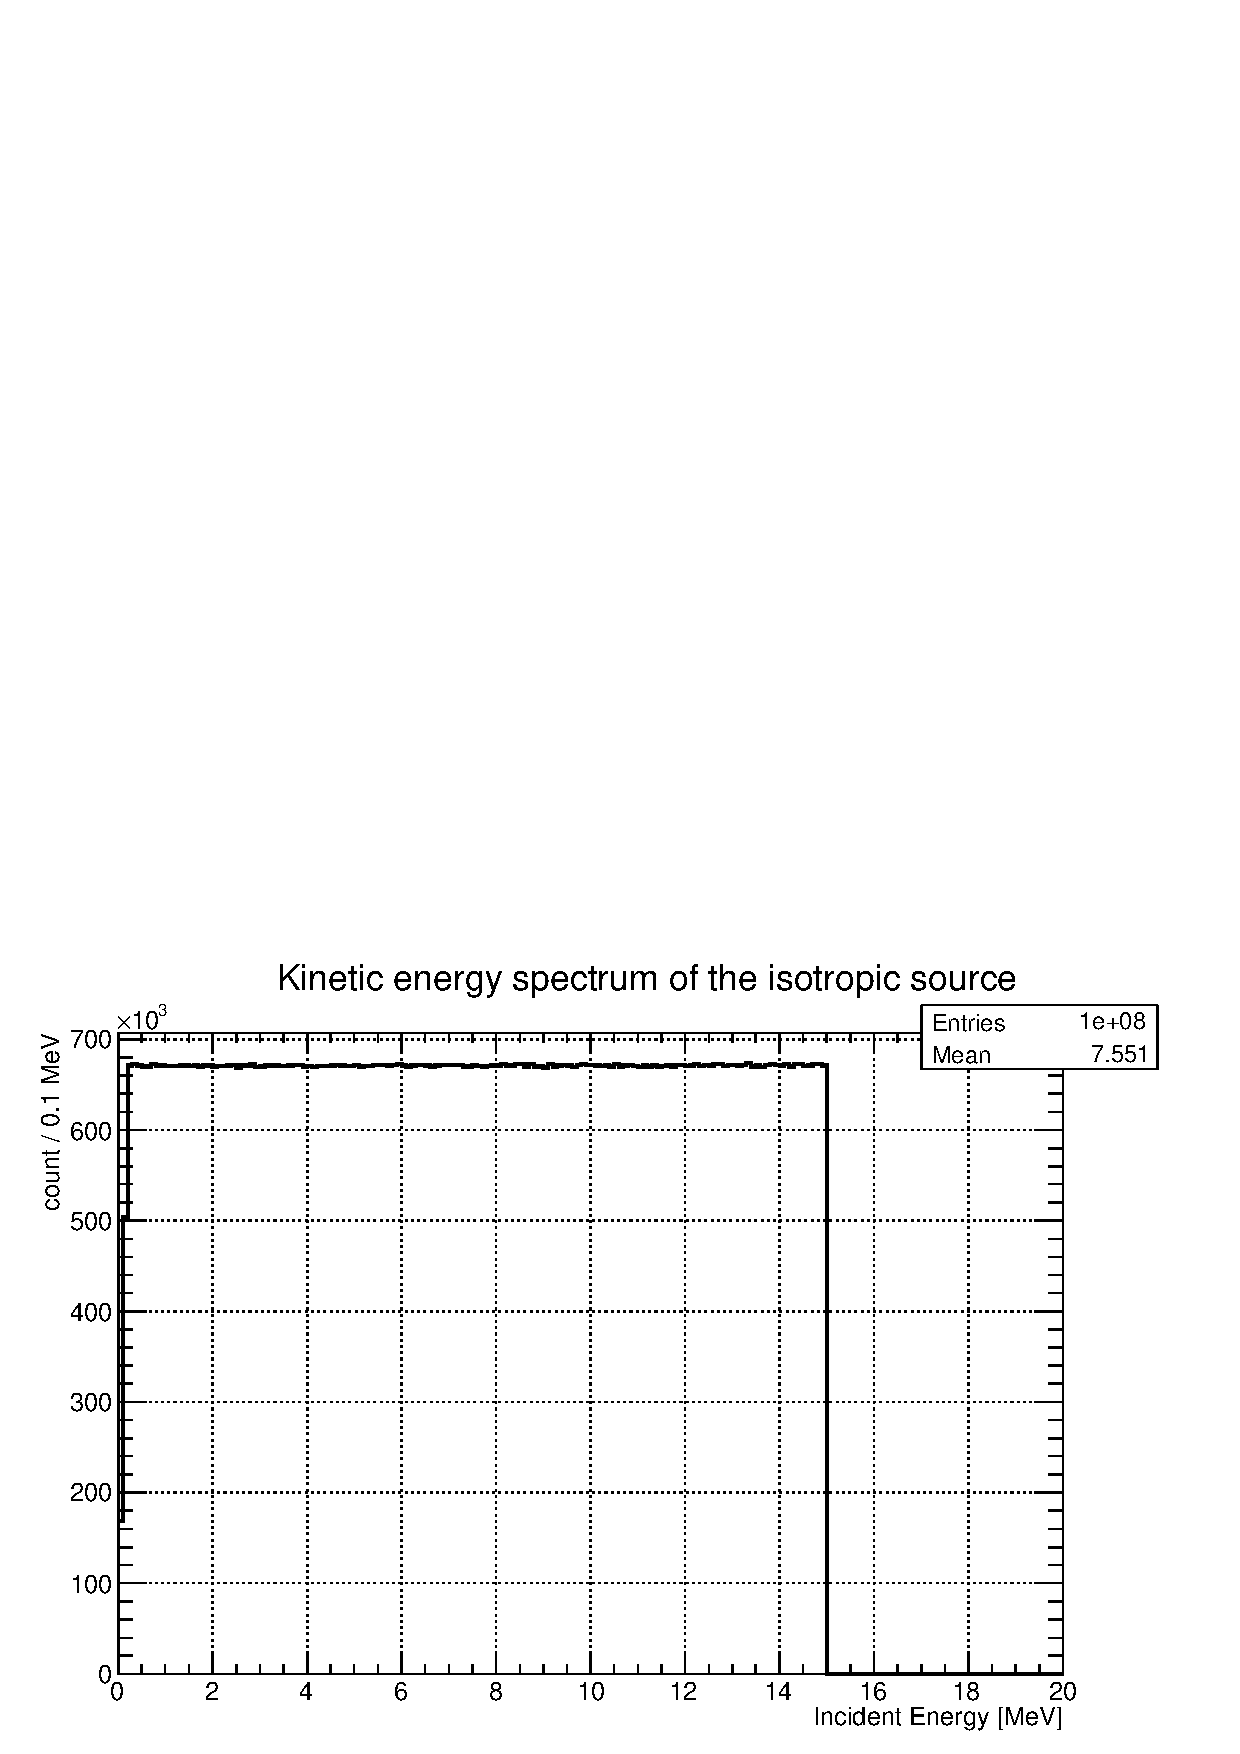
\includegraphics[width=100mm]{Chapter6/figures/kineticEnergySpectrum.png}
%\caption{Kinetic energy spectrum of the neutrons and gammas incident on the casing.}
%\label{fig:incidentEnergy}
%\end{center}
%\end{figure}

\begin{figure}[htbp]
\begin{center}
%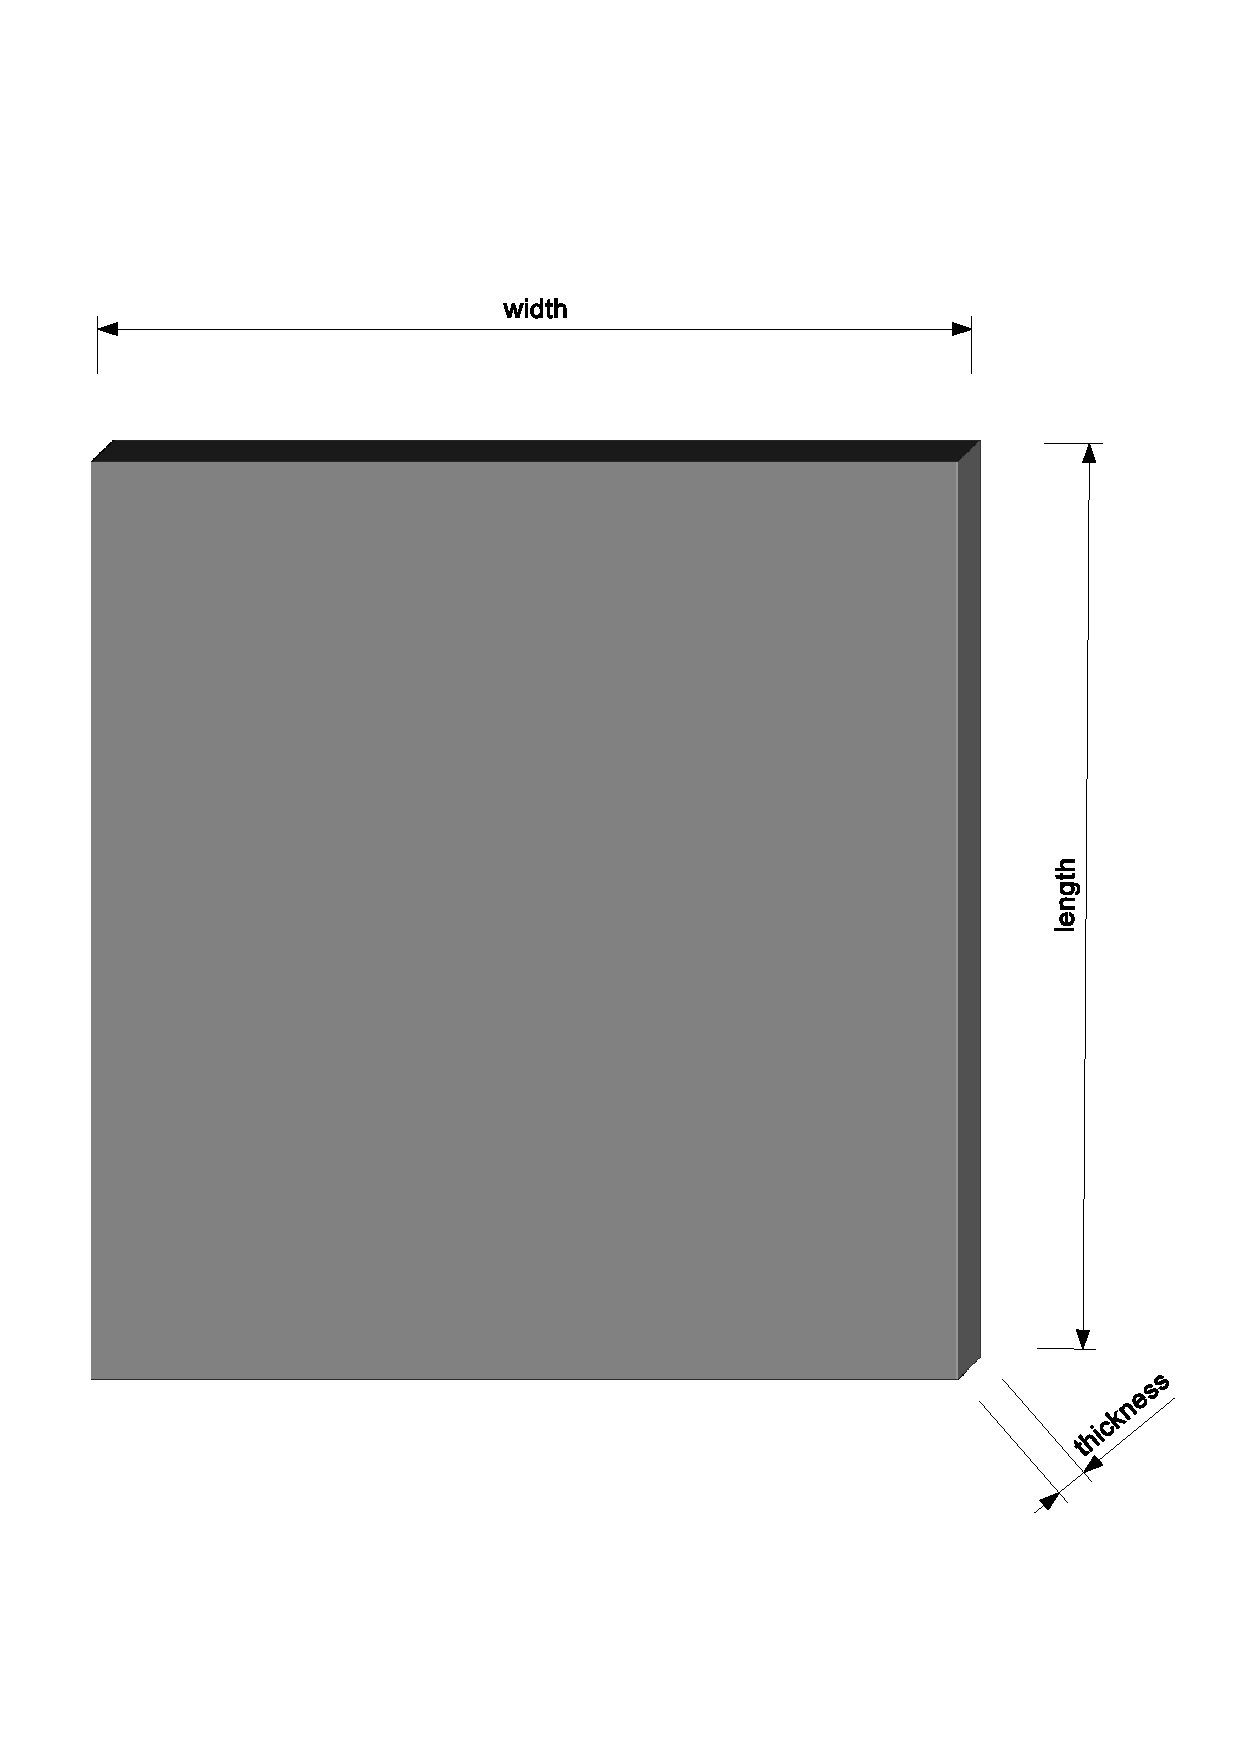
\includegraphics[width=60mm]{Chapter6/figures/casingDiagram1.png}
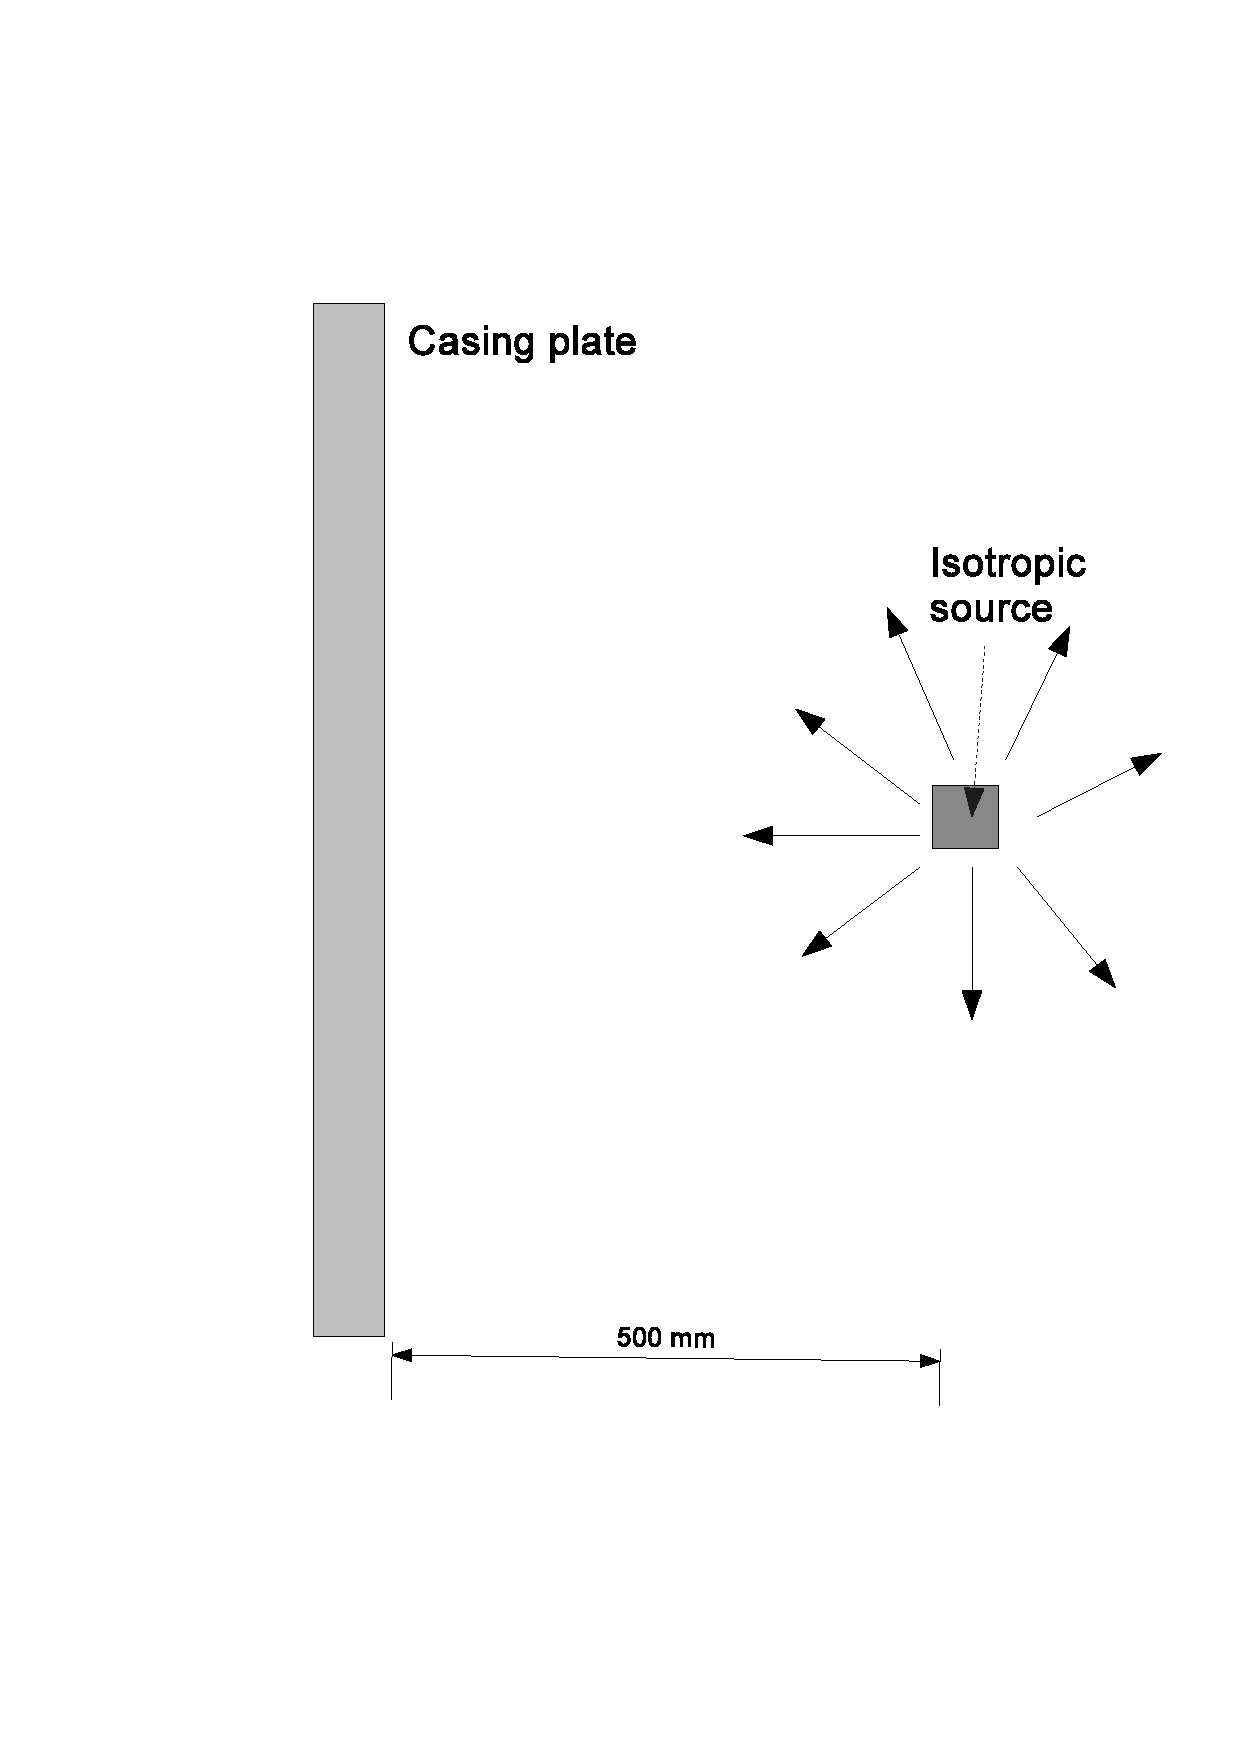
\includegraphics[width=120mm]{Chapter6/figures/setupDiagram1.png}
\caption{One layer of the casing plate of aluminium with dimension labels (left) and the experimental setup (right).}
\label{fig:casingDiagram}
\end{center}
\end{figure}
%----------------------------------------------------------------------------------------
%	SECTION 4- Efficiencies
%----------------------------------------------------------------------------------------

\subsection{Casing Efficiencies}
In order to quantify the effect of the detector casing, efficiencies are calculated on a energy binned basis. The efficiency $\epsilon$, as a function of incident kinetic energy is defined by equation~\ref{eq:efficiency}. 
\begin{equation}
\epsilon_{bin} = \frac{N_{p}^{bin}}{N_{T}^{bin}} = \frac{\textnormal{number of particles in energy bin that pass through casing}} {\textnormal{number of particles in energy bin that are incident on casing}}
\label{eq:efficiency}
\end{equation}
When a particle is incident on the detector it can either: not interact, scatter with forward momentum, scatter with backward momentum or be absorbed. Only particles that match the former two cases are considered successful. Particles that are then back scattered or absorbed do not pass the selection criteria. The efficiencies are then calculated from the particle counts for each kinetic energy bin.

\subsubsection{Examining Multiple Layers}
Depending on the detector array arrangement some detectors may encounter up to five layers of the casing in their path. It is then necessary to measure the effect that this would have on the energy spectra. To give a comparison of introducing additional layers, efficiencies as a function of incident energy for numbers of 1,2,3,4 and 5 layers are shown in figure \ref{fig:efficienciesAlLayers}. With energies of 2 MeV and below of particular interest, efficiencies in this range are shown separately in figure \ref{fig:efficienciesAlLayersZoom}.

\begin{figure}[htbp]
\begin{center}
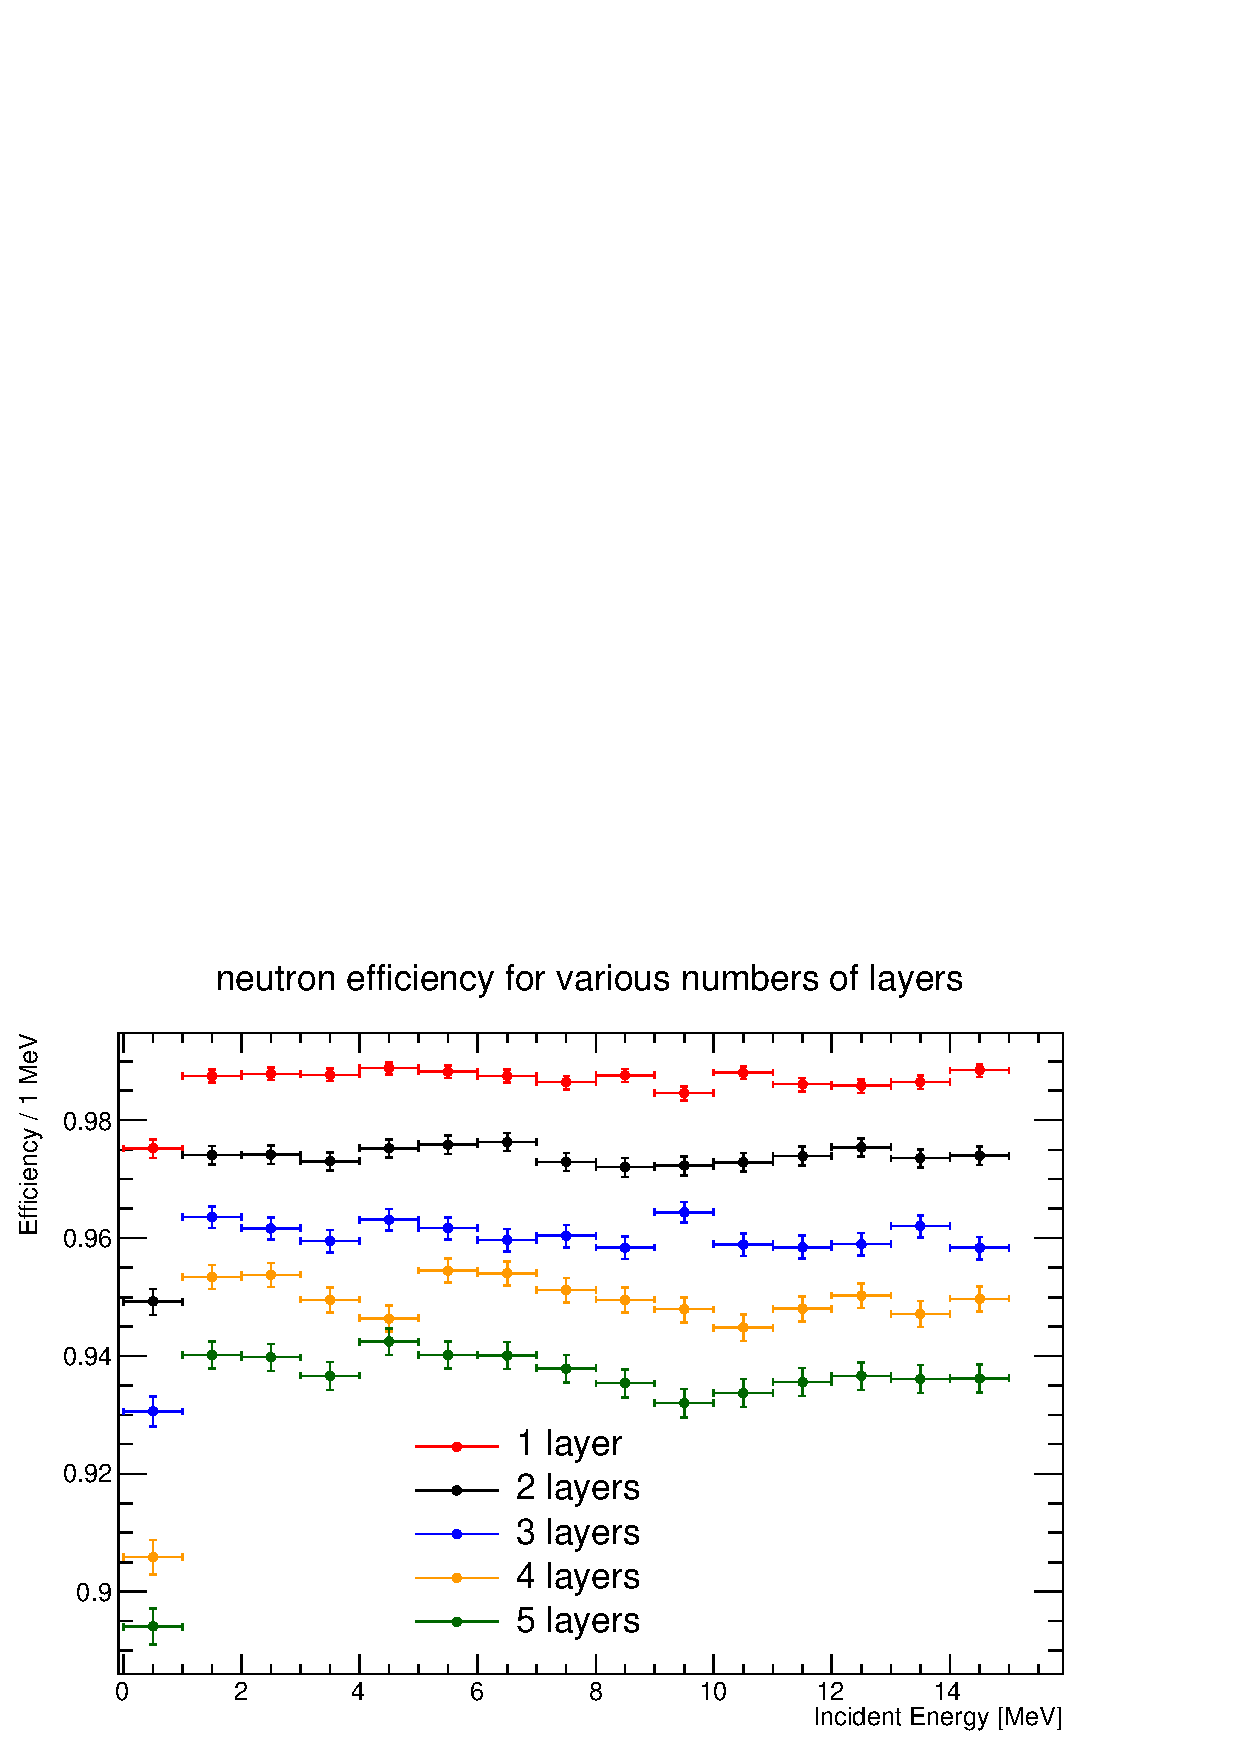
\includegraphics[width=75mm]{Chapter6/figures/neutronAlLayersEfficiency0-16MeV.png}
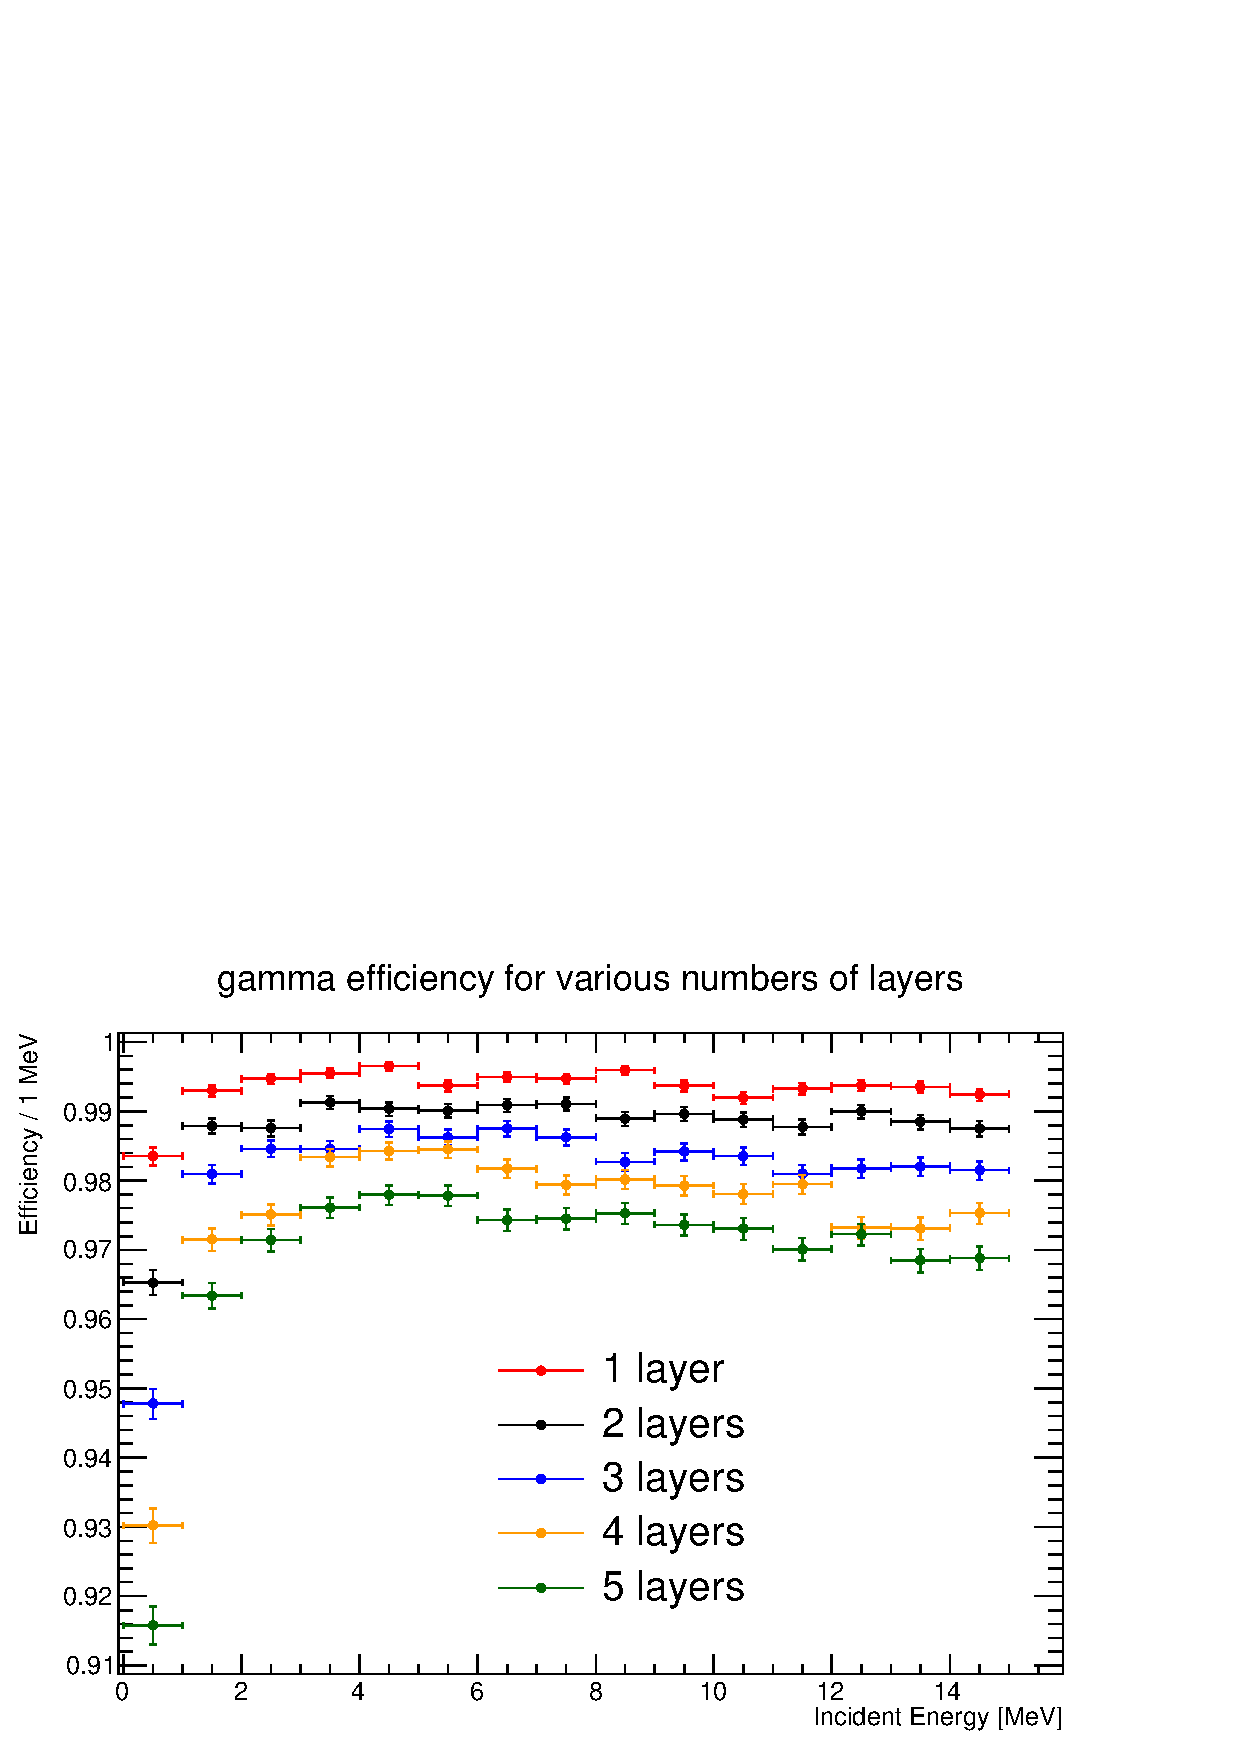
\includegraphics[width=75mm]{Chapter6/figures/gammaAlLayersEfficiency0-16MeV.png}
\caption{The neutron (left) and gamma (right) efficiencies for 1,2,3,4 and 5 layers of the aluminium casing.}
\label{fig:efficienciesAlLayers}
\end{center}
\end{figure}

\begin{figure}[htbp]
\begin{center}
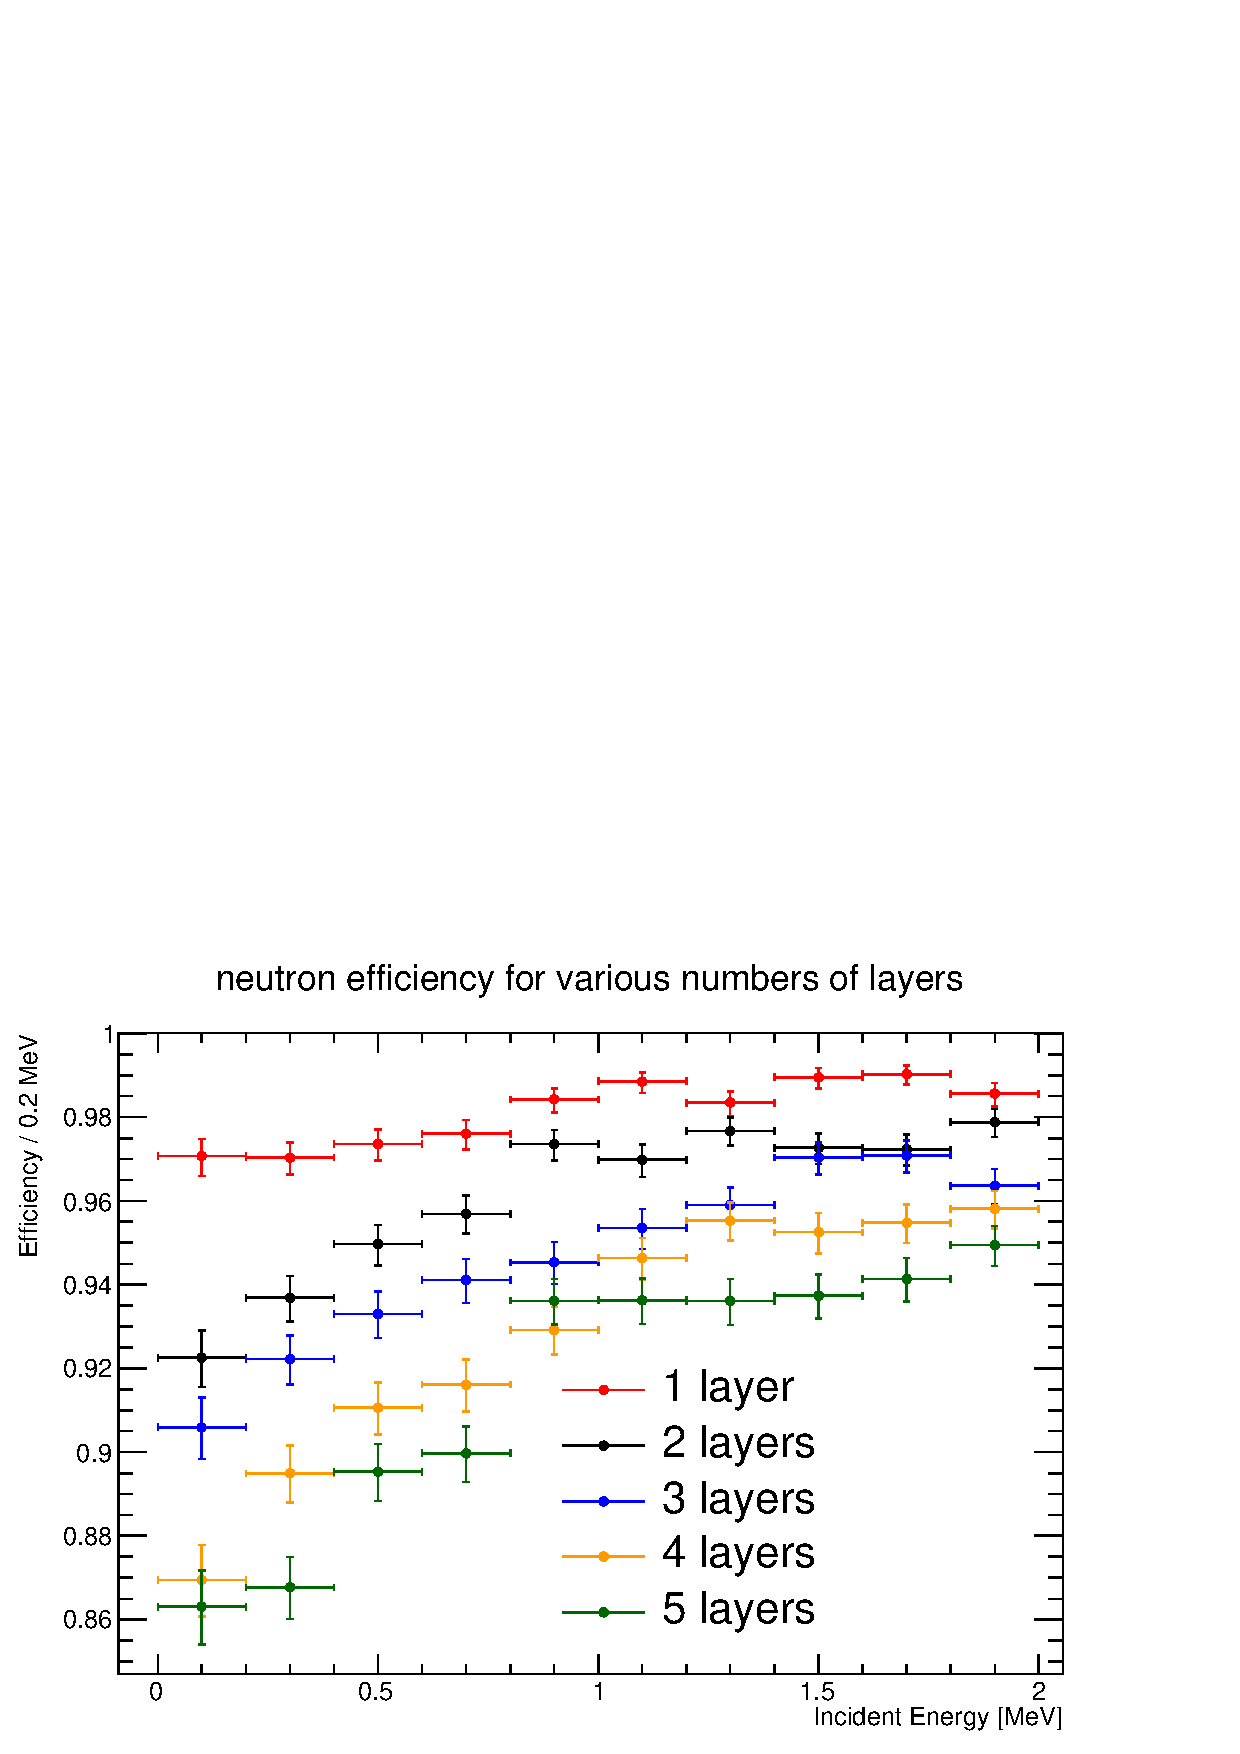
\includegraphics[width=75mm]{Chapter6/figures/neutronAlLayersEfficiency0-2MeV.png}
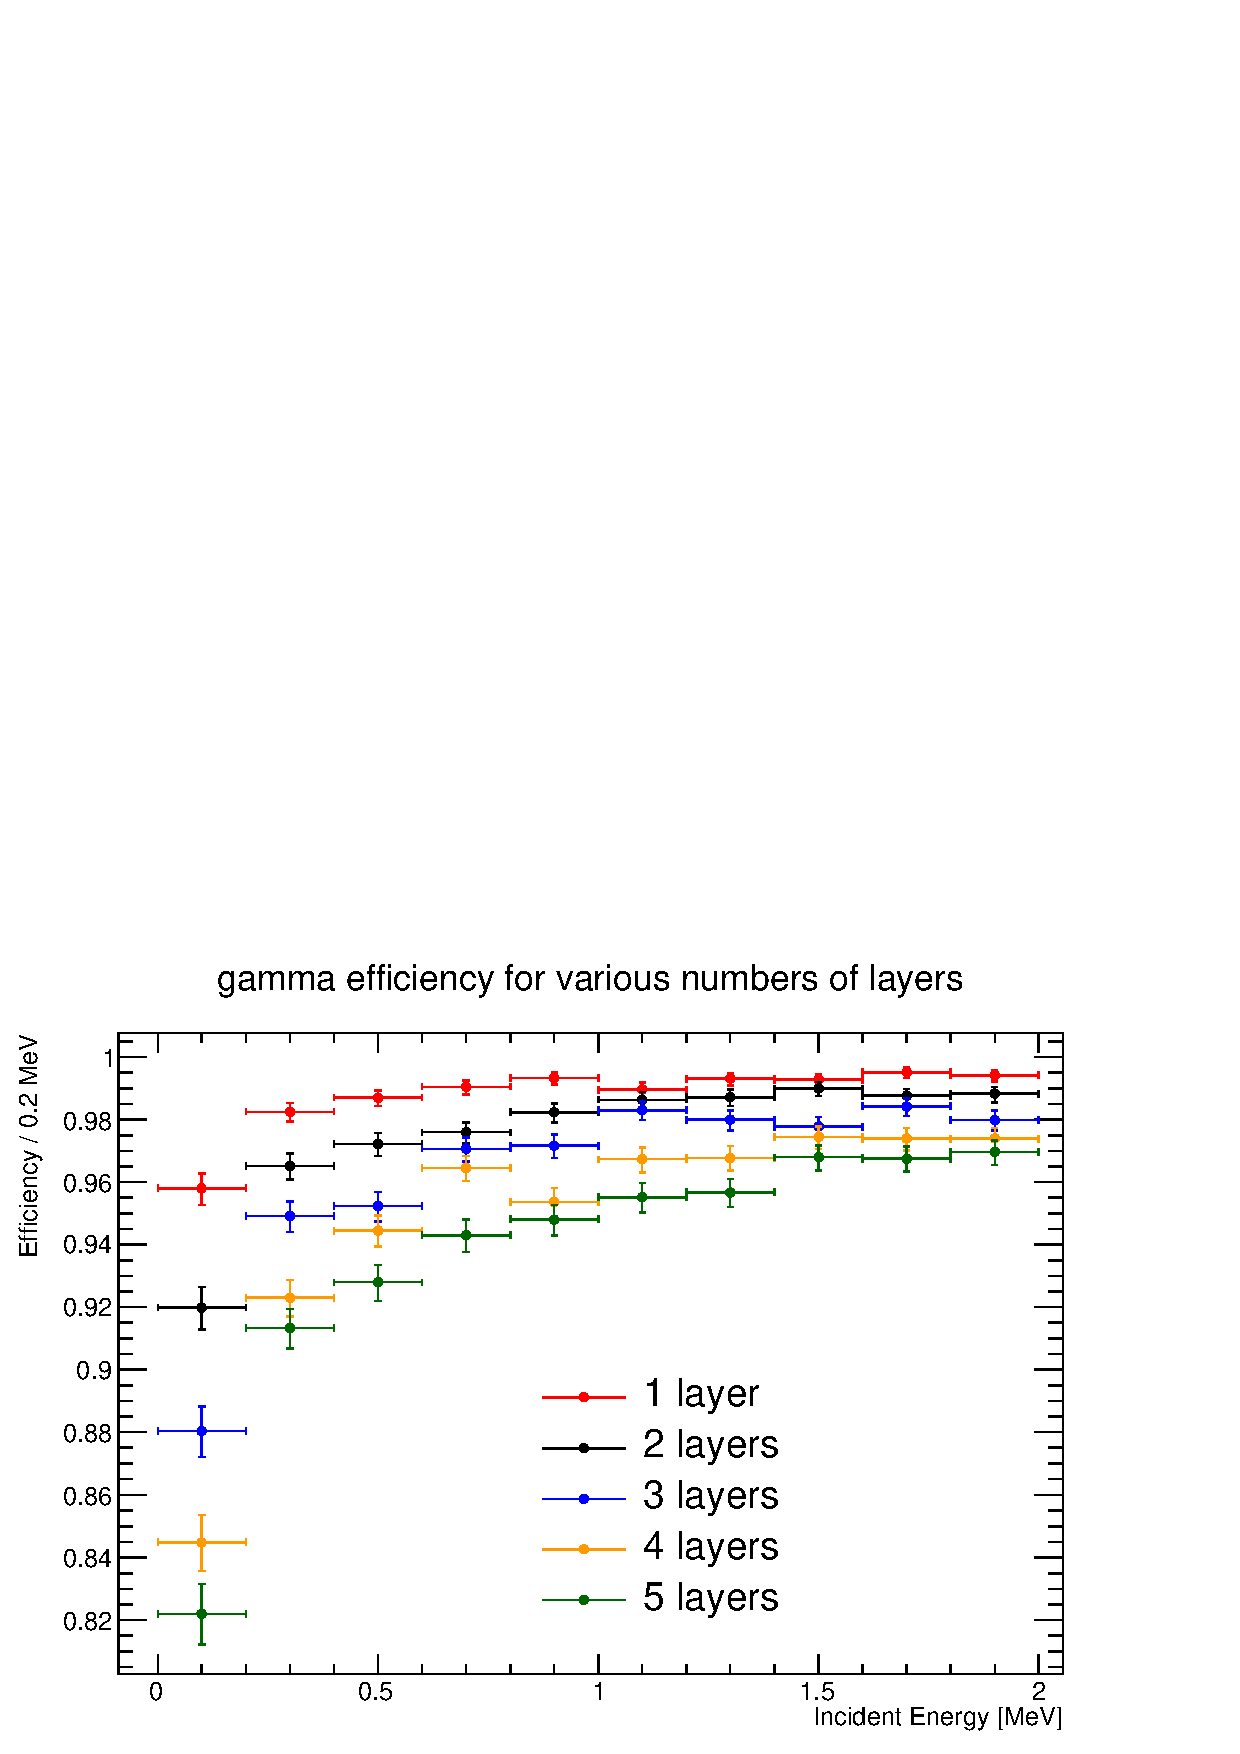
\includegraphics[width=75mm]{Chapter6/figures/gammaAlLayersEfficiency0-2MeV.png}
\caption{The neutron (left) and gamma (right) efficiencies for 1,2,3,4 and 5 layers of the aluminium casing in the energy region of 0 - 2 MeV.}
\label{fig:efficienciesAlLayersZoom}
\end{center}
\end{figure}

In can be noticed that neutron efficiencies can exceed 97\% for 1 layer of the aluminium casing. Similarly for photons efficiencies can surpass 98\% when the <100 keV regime is excluded. In this low energy region it falls to just below 96\% however. Both particles show efficiencies that are largely independent of the incident energy but with it slightly improving at energies above 1 MeV. When considering 5 layers of the material these efficiencies are reduced to $\sim$94\% and $\sim$97\% for neutrons and gammas respectively for energies above 1 MeV. In the case for particles <1 MeV, efficiencies fall to as low as 86\% for neutrons and 82\% for gammas.

It is important to realise that due to kinematic restrictions from elastic scattering, neutrons can only transfer up to 14\% of their kinetic energy per scatter on aluminium, calculated using equation \ref{eq:neutronScatter}. This can be noticed when taking the ratio of the kinetic energy of incident neutrons to the kinetic energy of the neutrons leaving the casing, shown left in figure~\ref{fig:energyRatio}. For photons however no such kinematic restrictions exist on elastic scattering, shown right in figure~\ref{fig:energyRatio}.

\begin{figure}[htbp]
\begin{center}
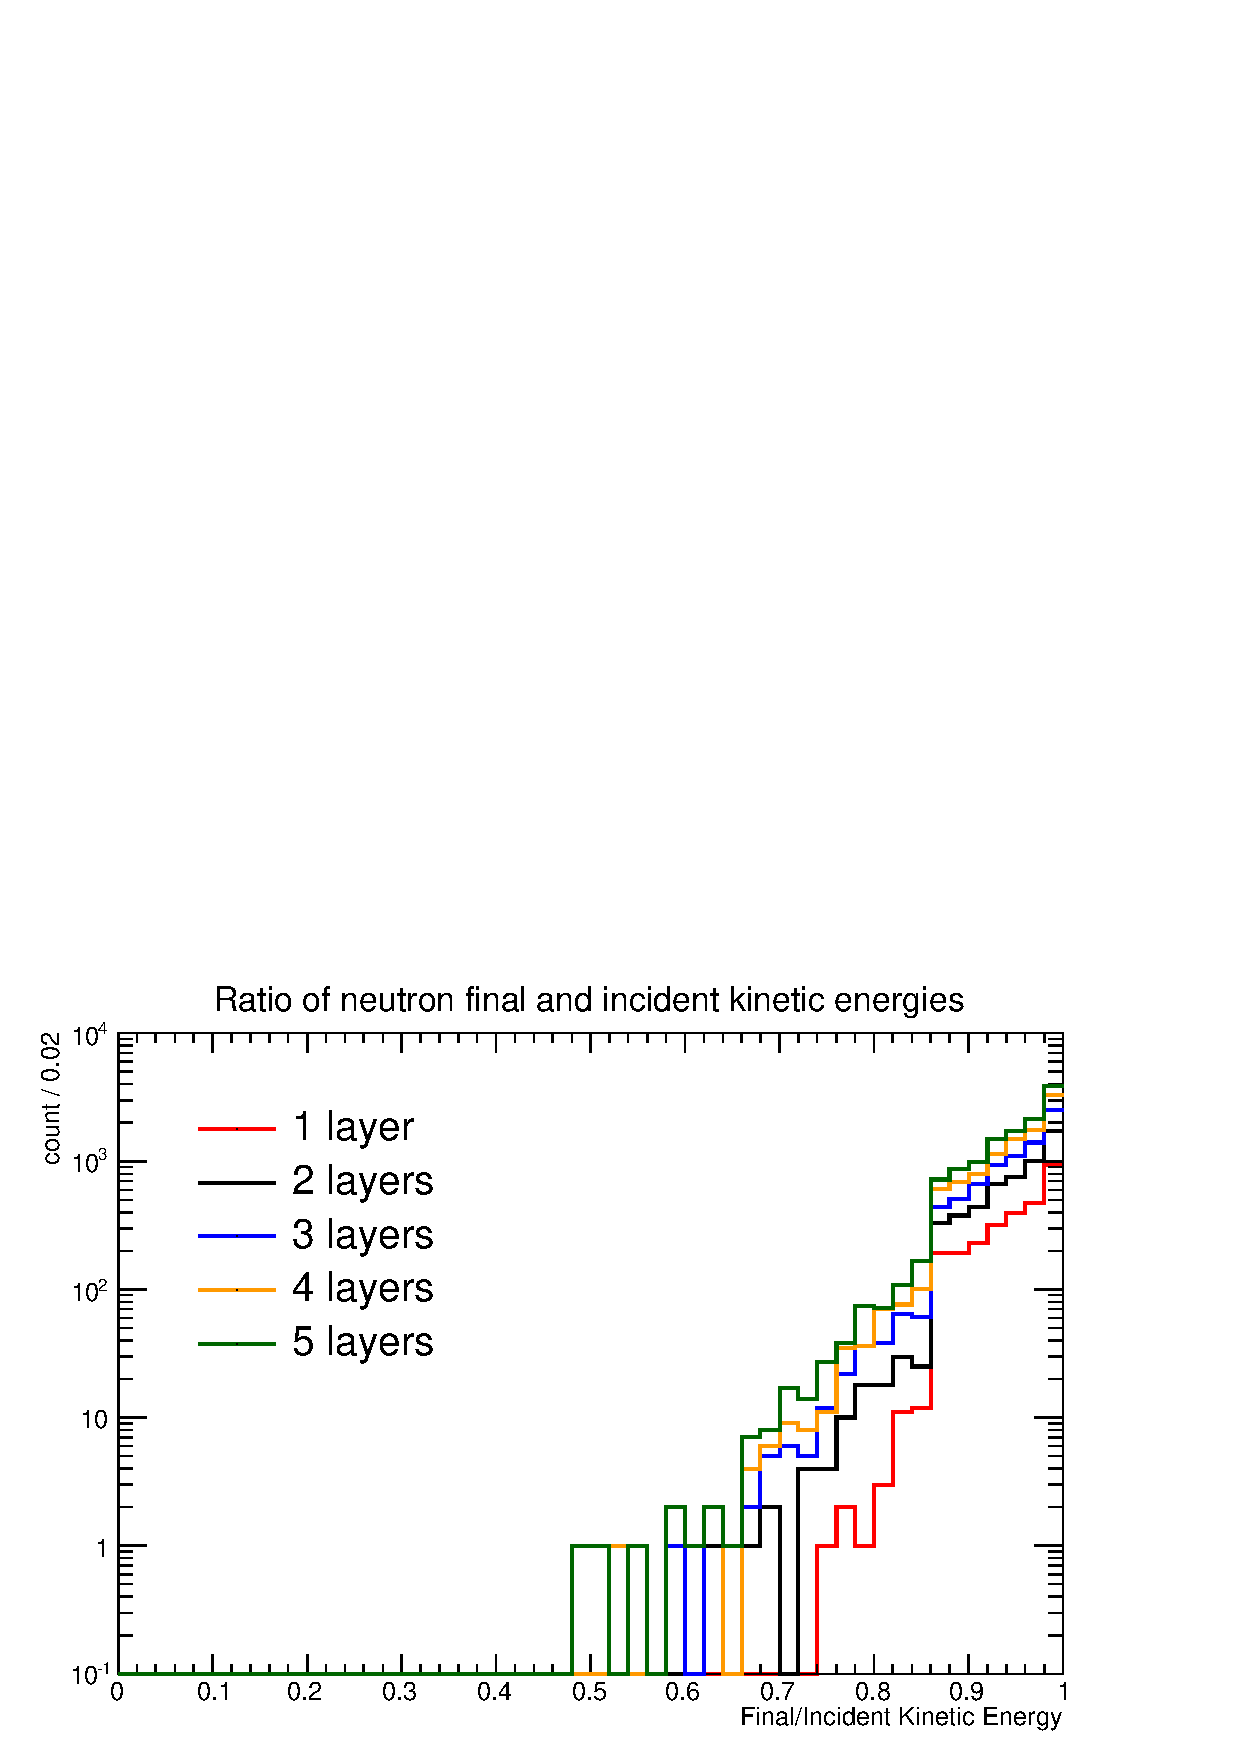
\includegraphics[width=75mm]{Chapter6/figures/neutronAlLayersEnergyRatio.png}
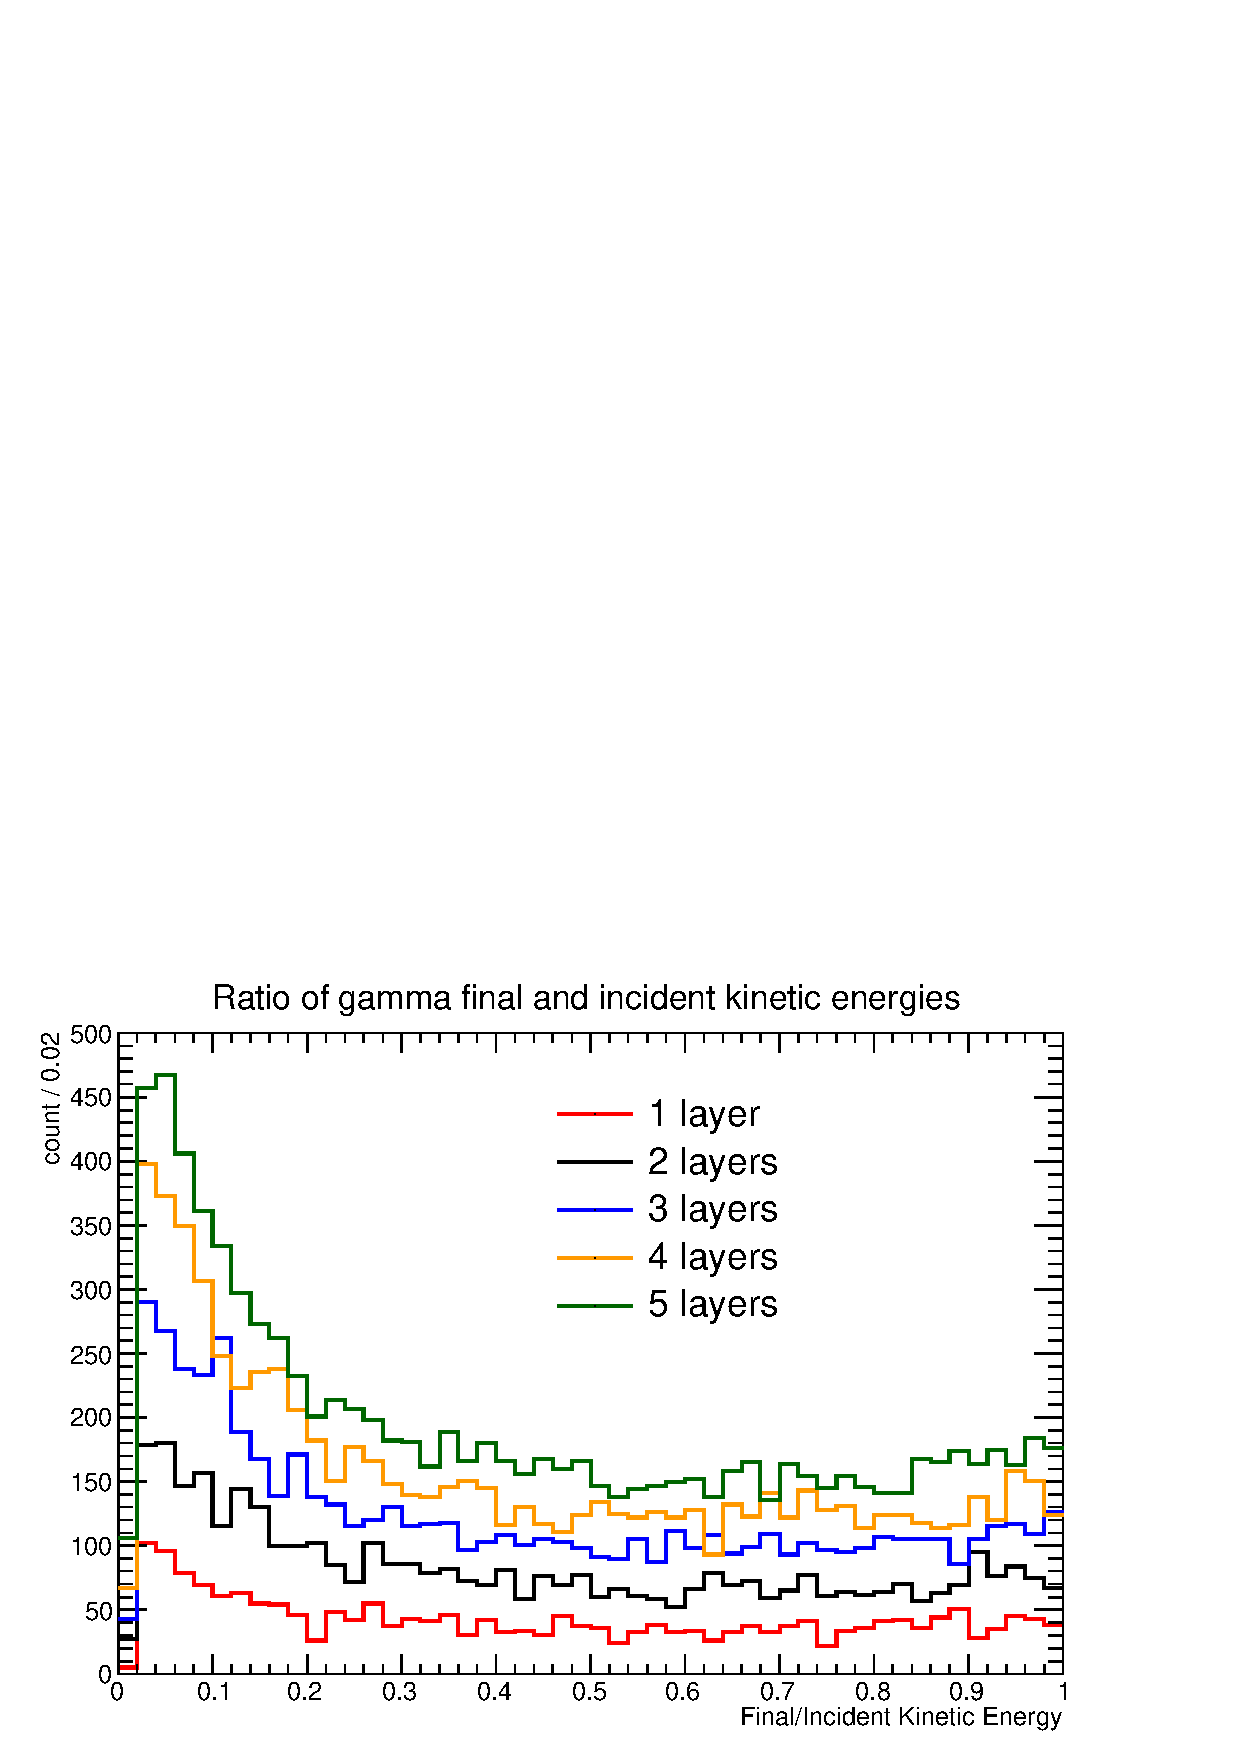
\includegraphics[width=75mm]{Chapter6/figures/gammaAlLayersEnergyRatio.png}
\caption{The ratio of kinetic energies for the neutrons (left) and gammas (right) upon leaving the casing to entering it for 1,2,3,4 and 5 layers of the casing. The dashed line on the neutron plot indicates the maximum possible energy transfer from one scatter of 14\%.}
\label{fig:energyRatio}
\end{center}
\end{figure}

\subsubsection{Other Materials}
Some of the other potential candidates for casing materials are also implemented for comparison. The two other materials tested are carbon fiber (C$_{3}$H$_{3}$N), density of 1.8 gcm$^{-3}$ and Iron (100\% $^{56}_{26}$Fe), density of 7.87 gcm$^{-3}$. These are tested for casings of 1,3 and 5 mm thicknesses against aluminium, density 2.7 gcm$^{-3}$. Their associated efficiencies are shown in figure \ref{fig:efficienciesMaterial}, with separate efficiencies calculated for the lower energy range of 0 to 2 MeV in figure \ref{fig:efficienciesMaterialZoom}. 

\begin{figure}[htbp]
\begin{center}
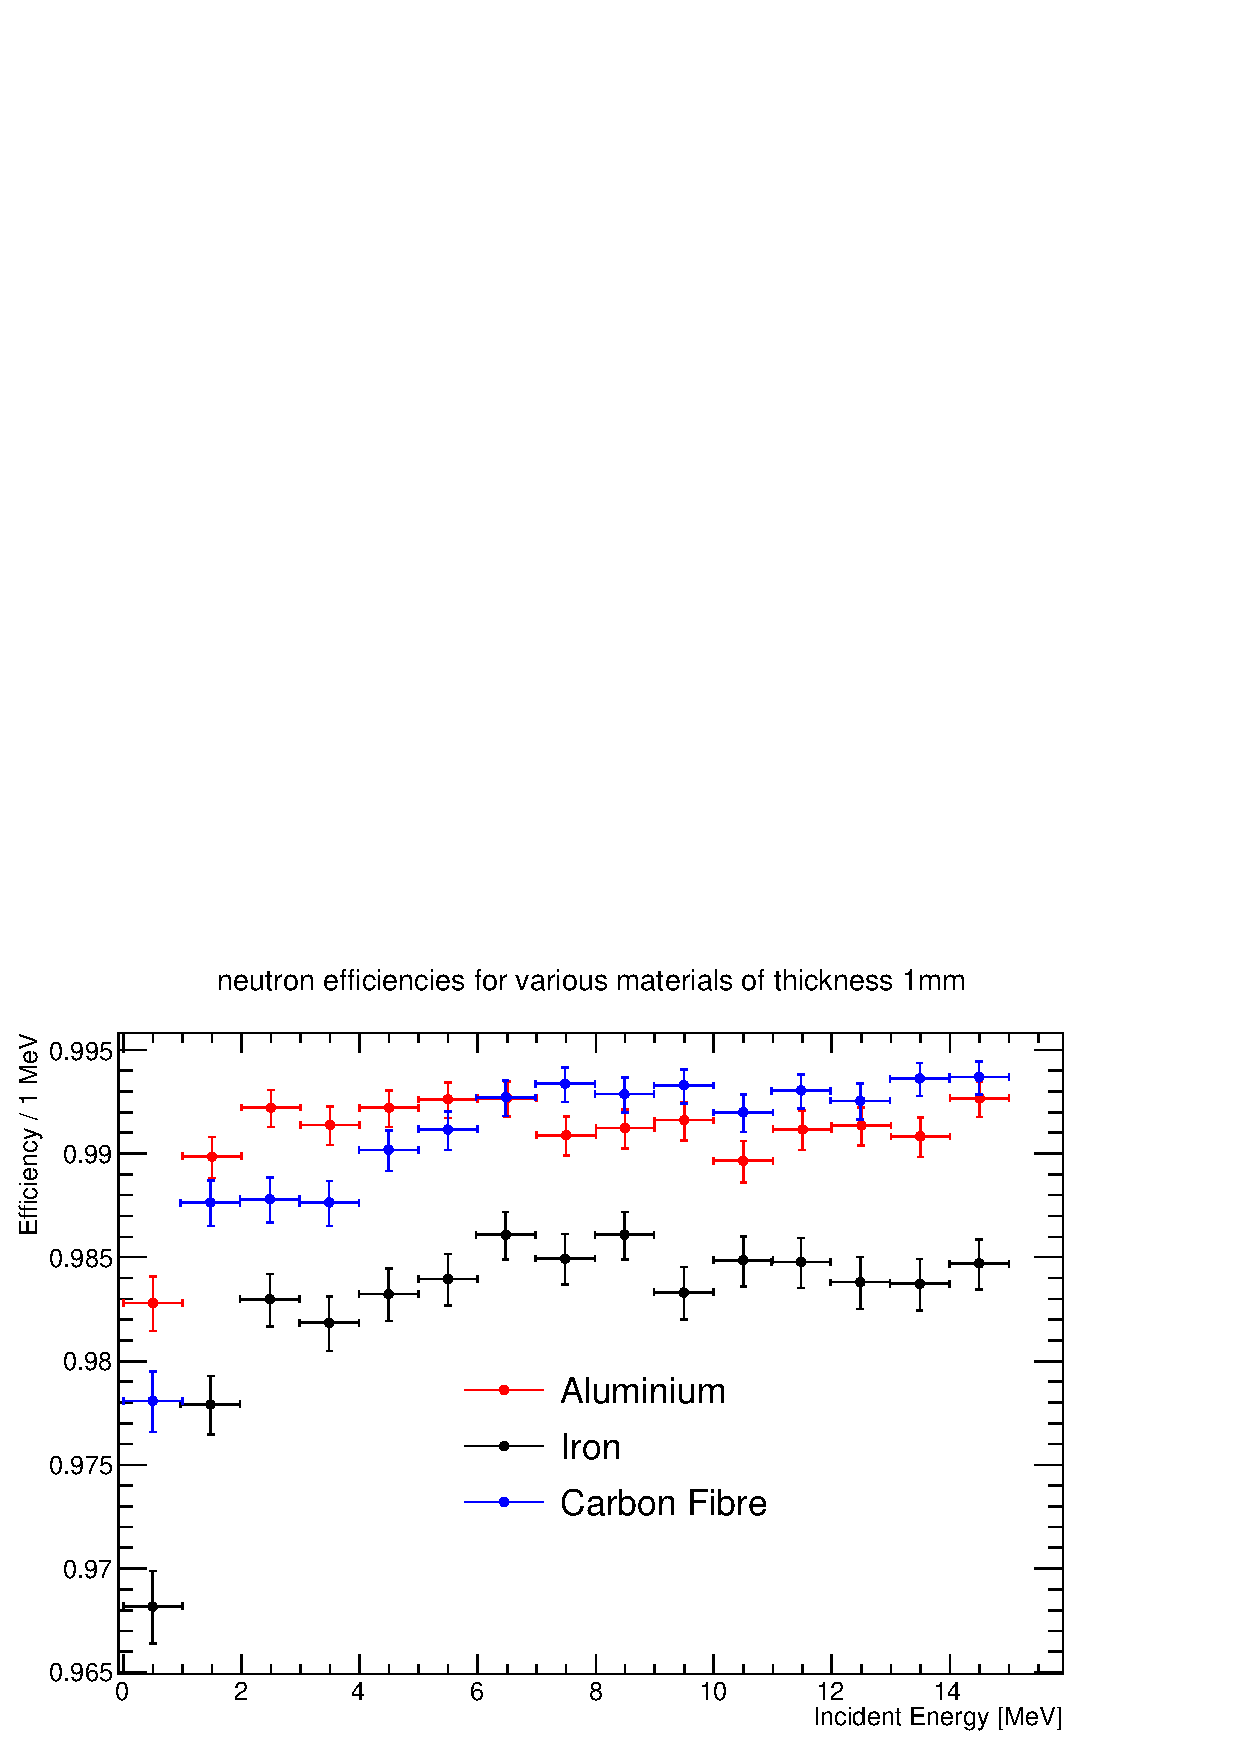
\includegraphics[width=75mm]{Chapter6/figures/neutron1mmMaterialsEfficiency0-16MeV.png}
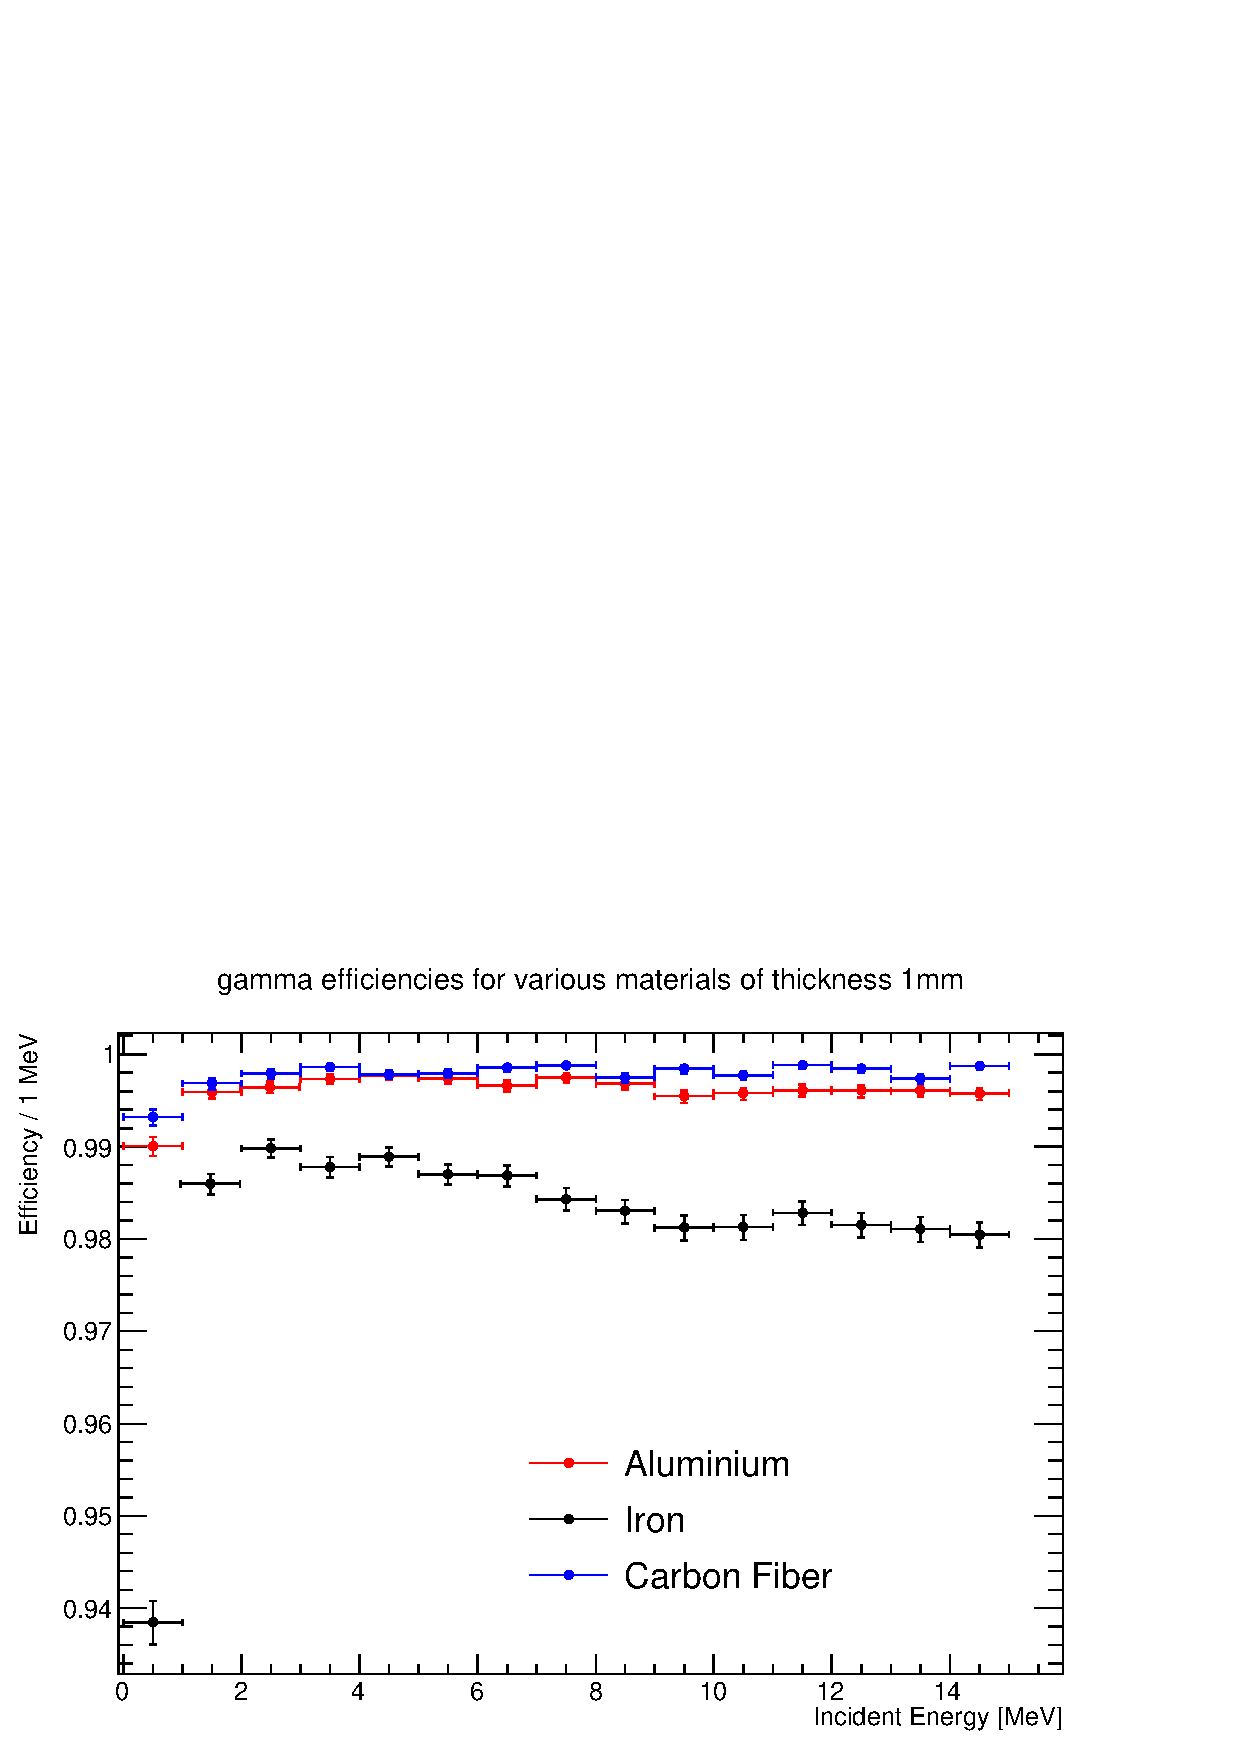
\includegraphics[width=75mm]{Chapter6/figures/gamma1mmMaterialsEfficiency0-16MeV.png}
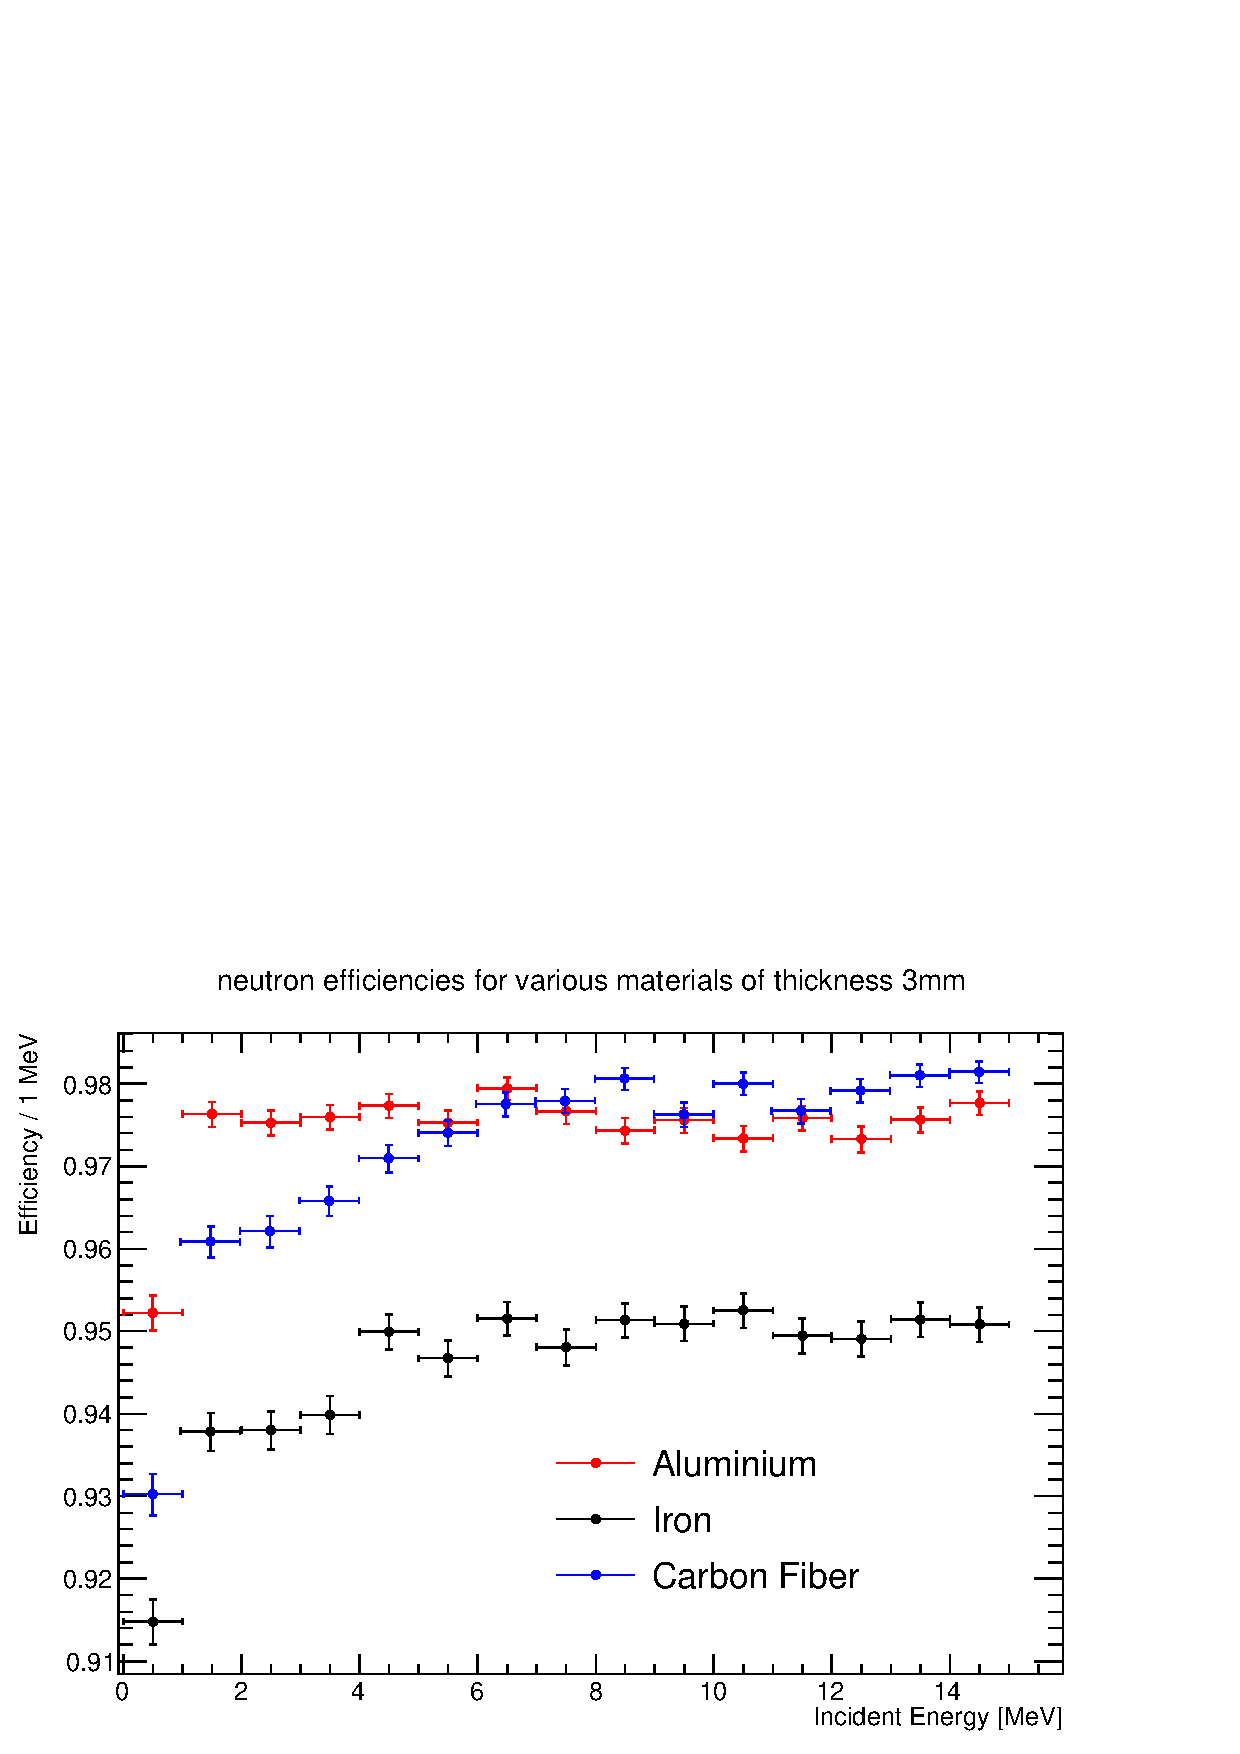
\includegraphics[width=75mm]{Chapter6/figures/neutron3mmMaterialsEfficiency0-16MeV.png}
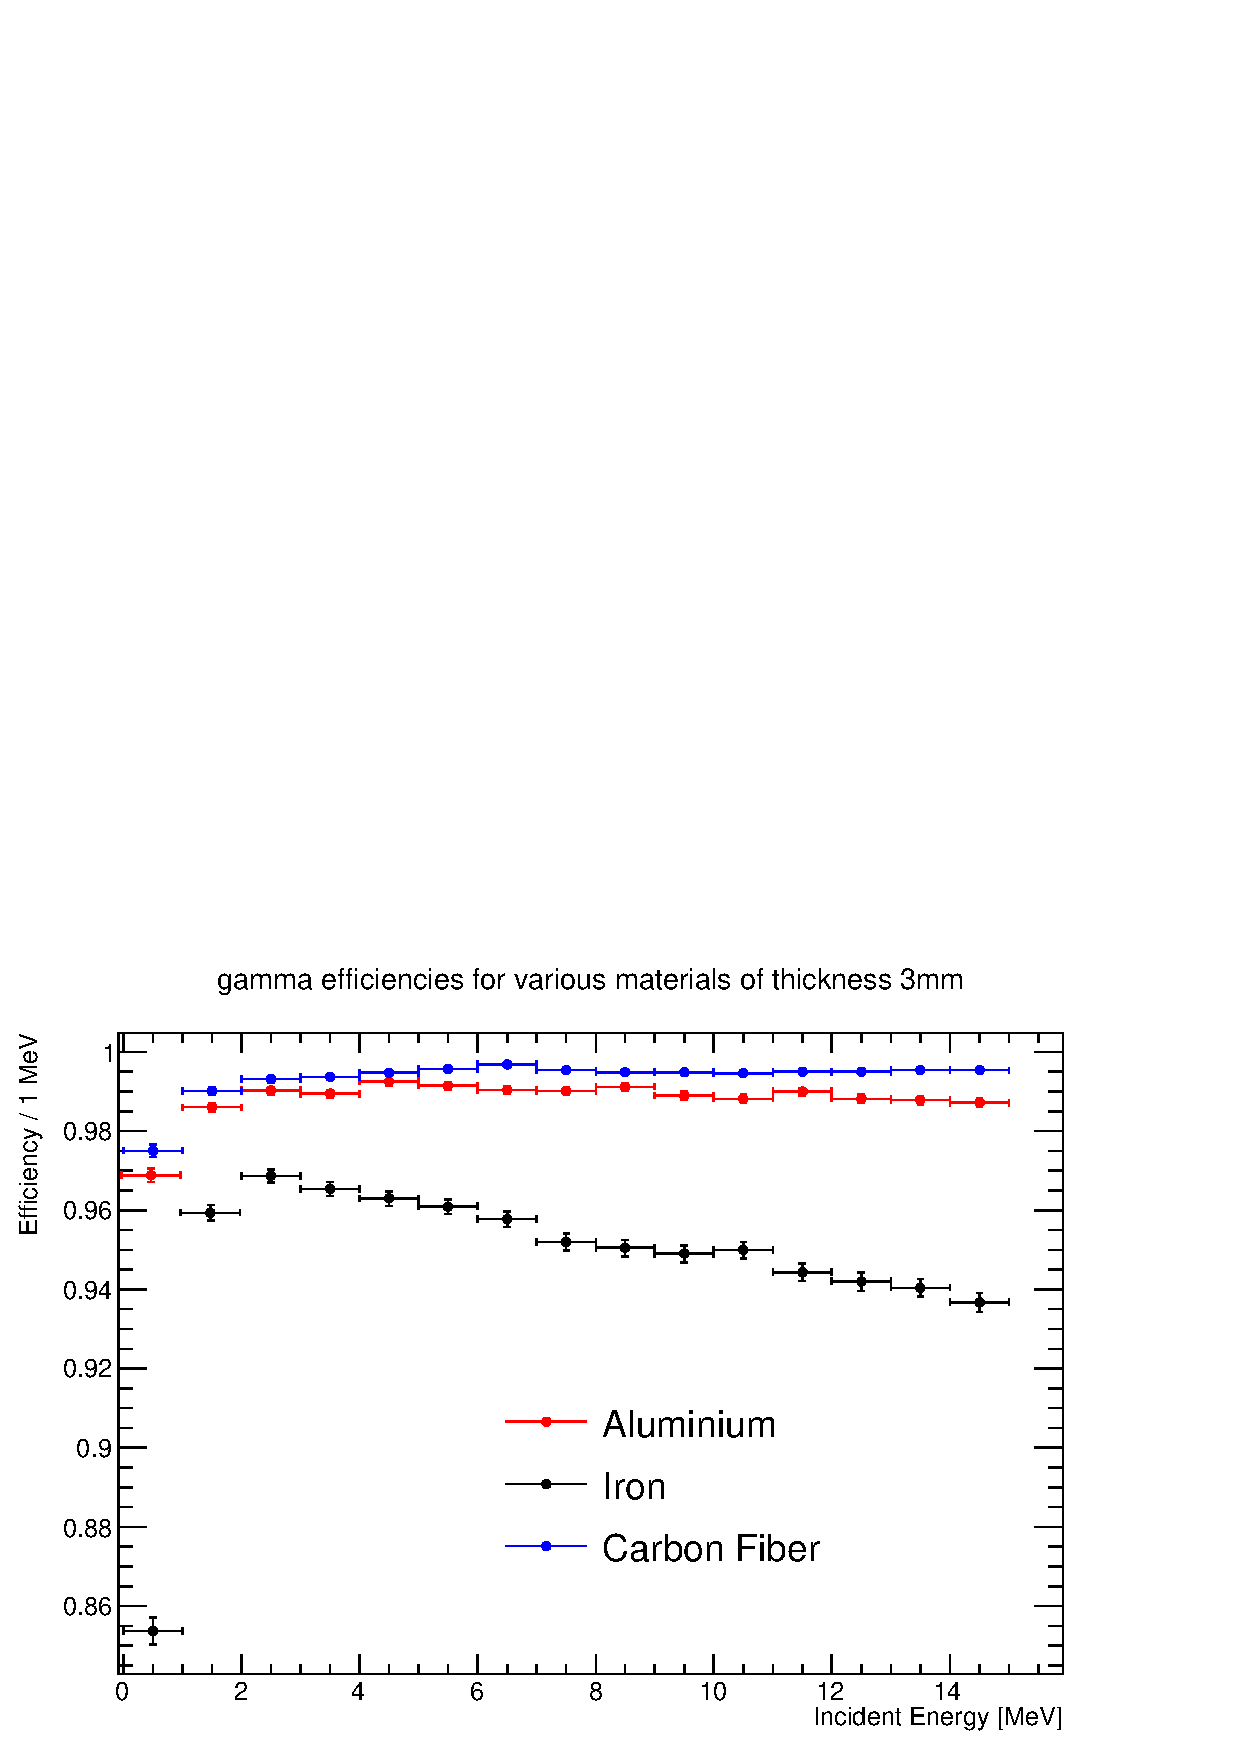
\includegraphics[width=75mm]{Chapter6/figures/gamma3mmMaterialsEfficiency0-16MeV.png}
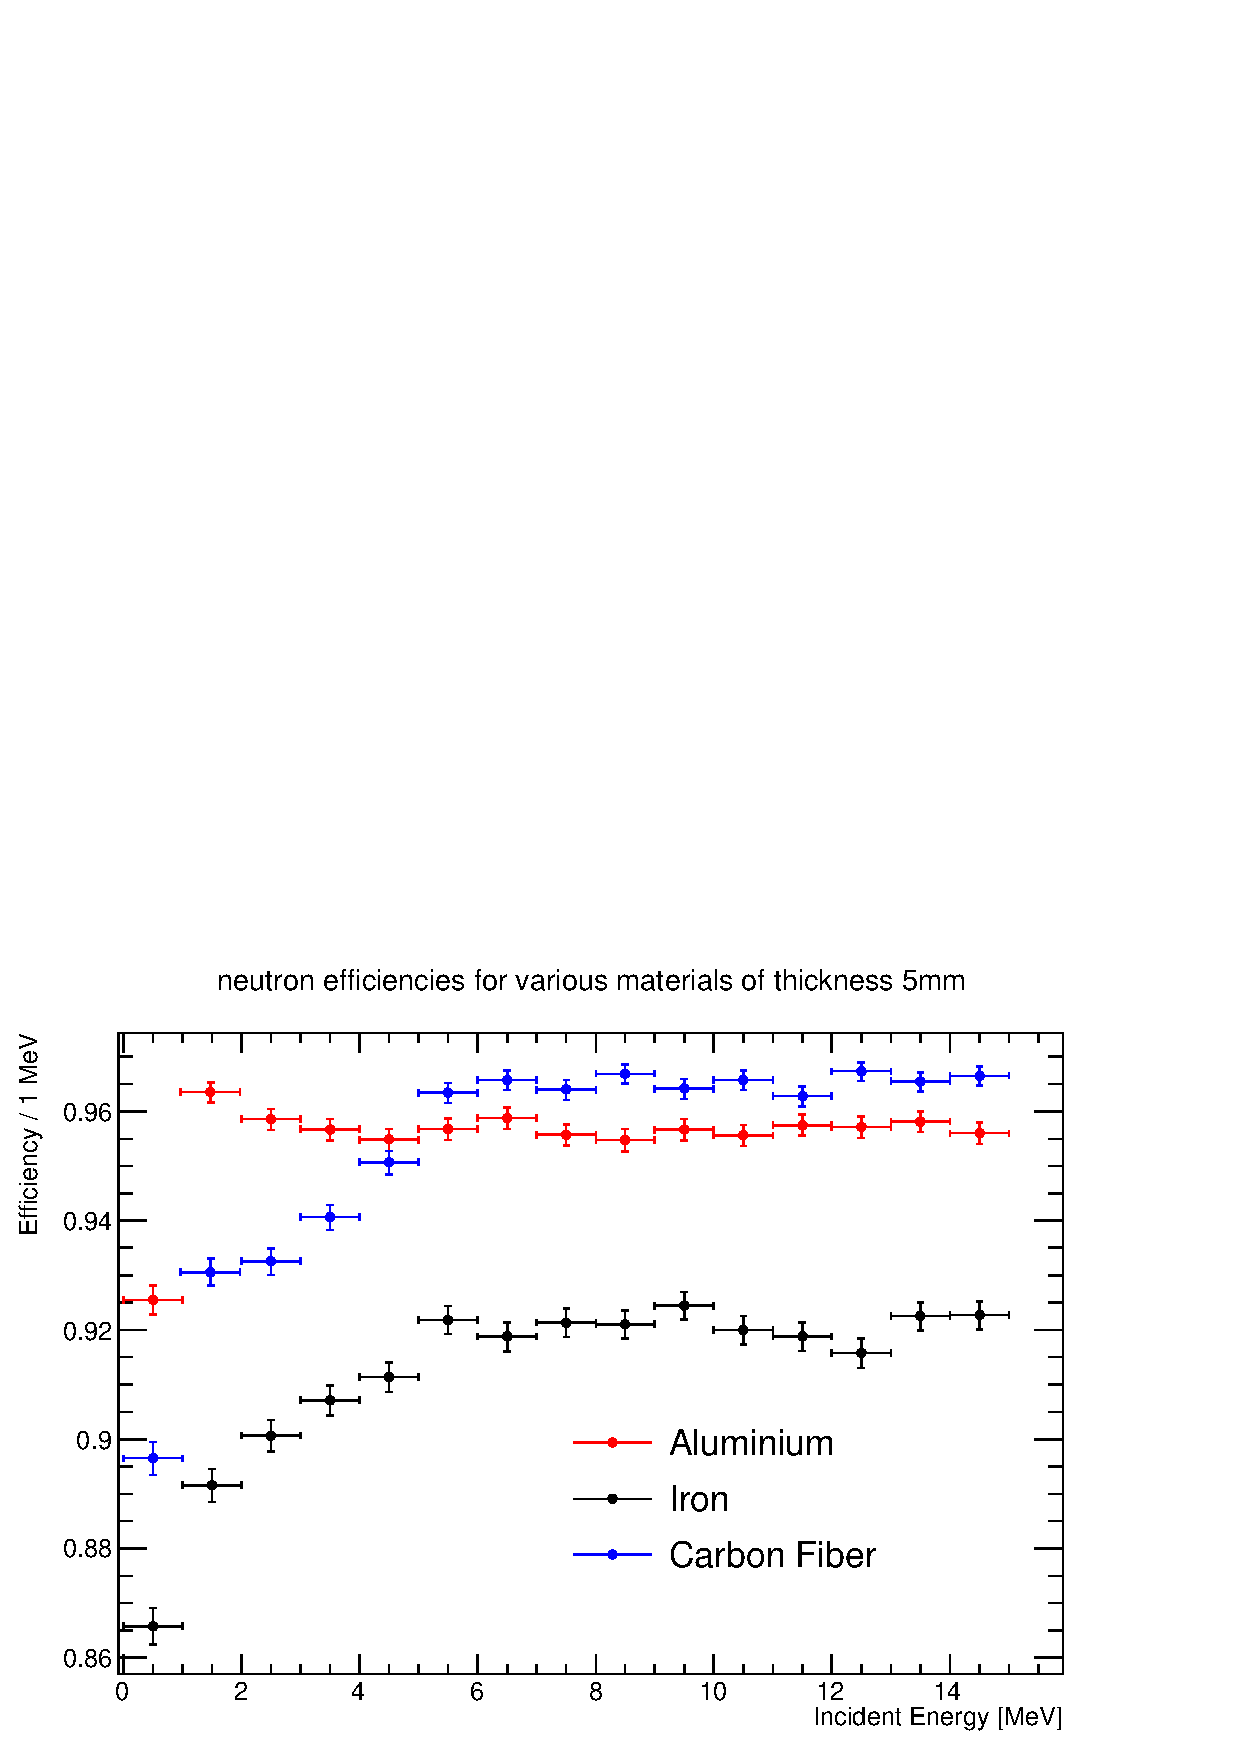
\includegraphics[width=75mm]{Chapter6/figures/neutron5mmMaterialsEfficiency0-16MeV.png}
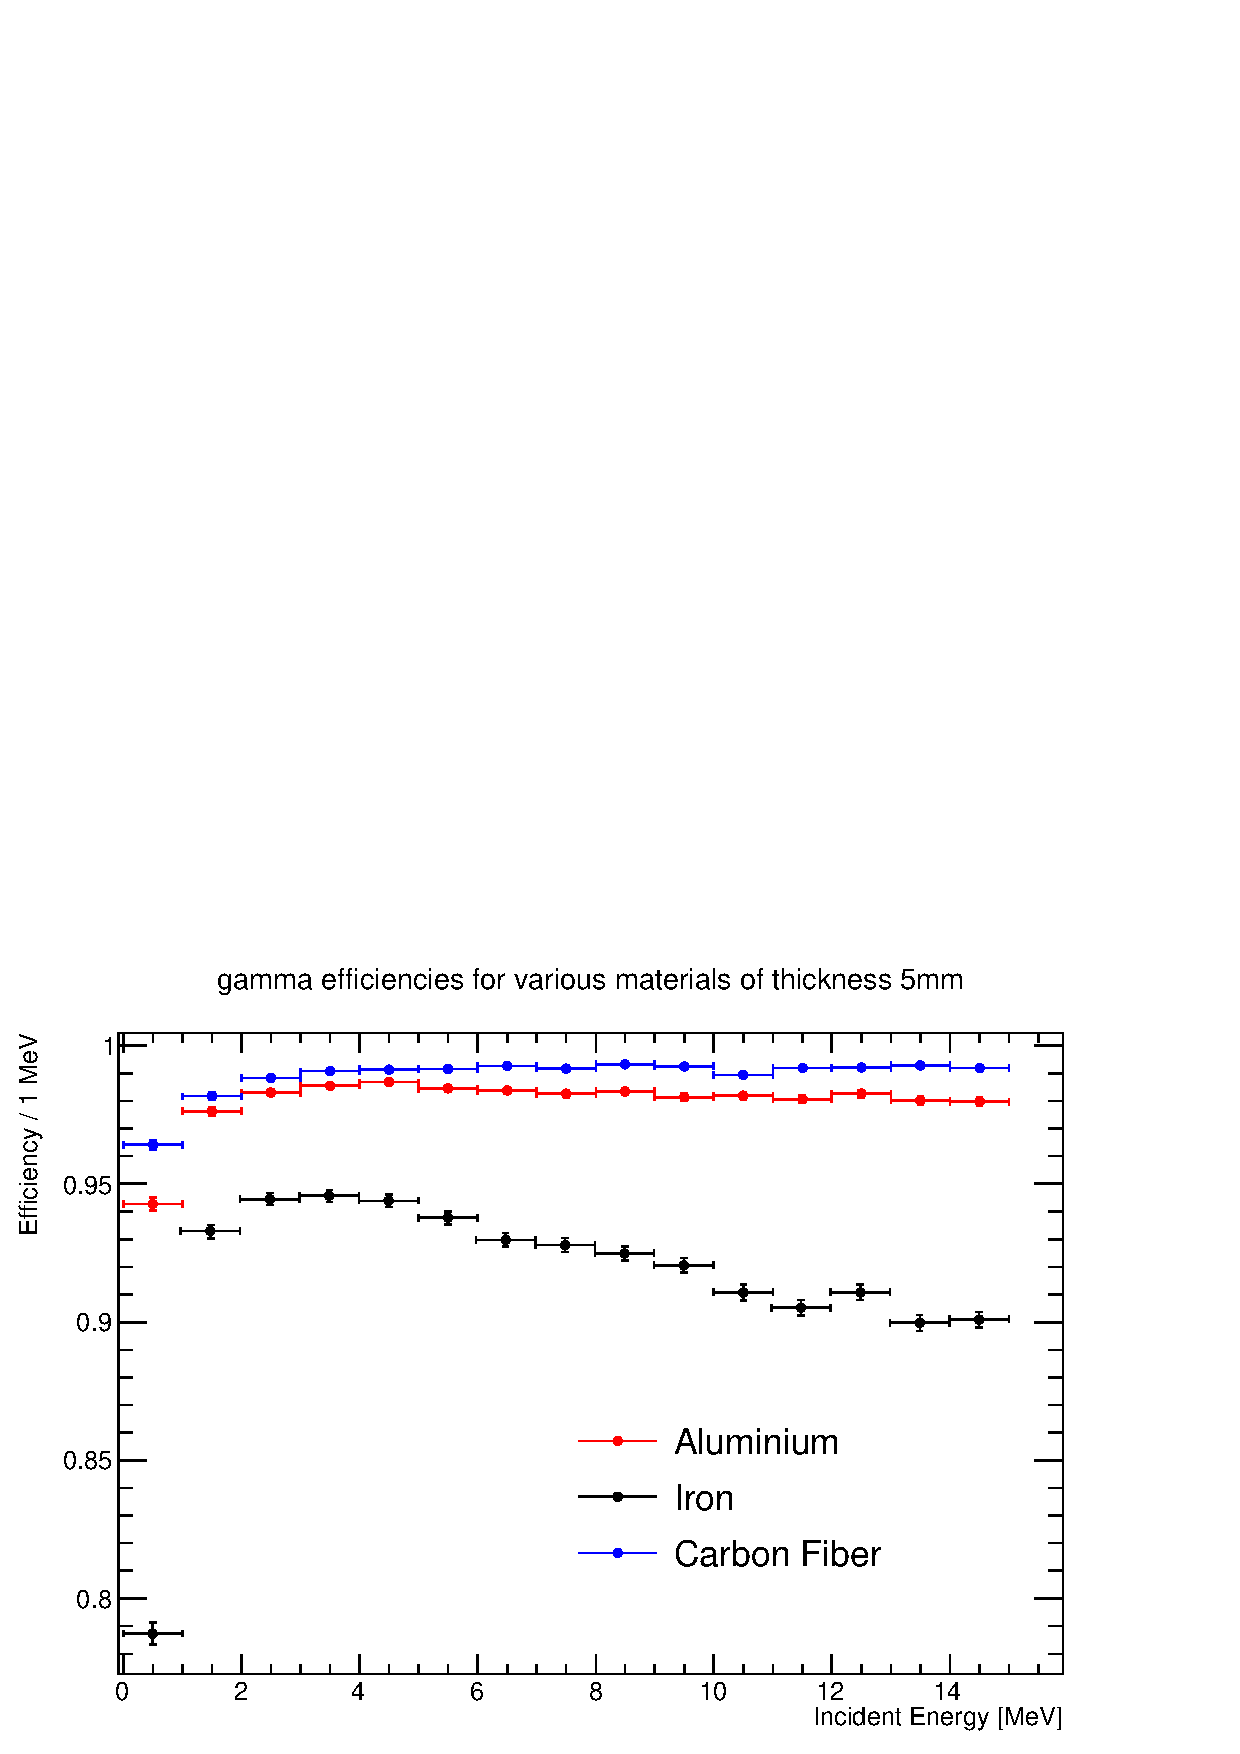
\includegraphics[width=75mm]{Chapter6/figures/gamma5mmMaterialsEfficiency0-16MeV.png}
\caption{The neutron (left) and gamma (right) efficiencies for carbon fibre, Iron and aluminium casings of 1 (top), 3 (middle) and 5 mm (bottom) thicknesses.}
\label{fig:efficienciesMaterial}
\end{center}
\end{figure}

\begin{figure}[htbp]
\begin{center}
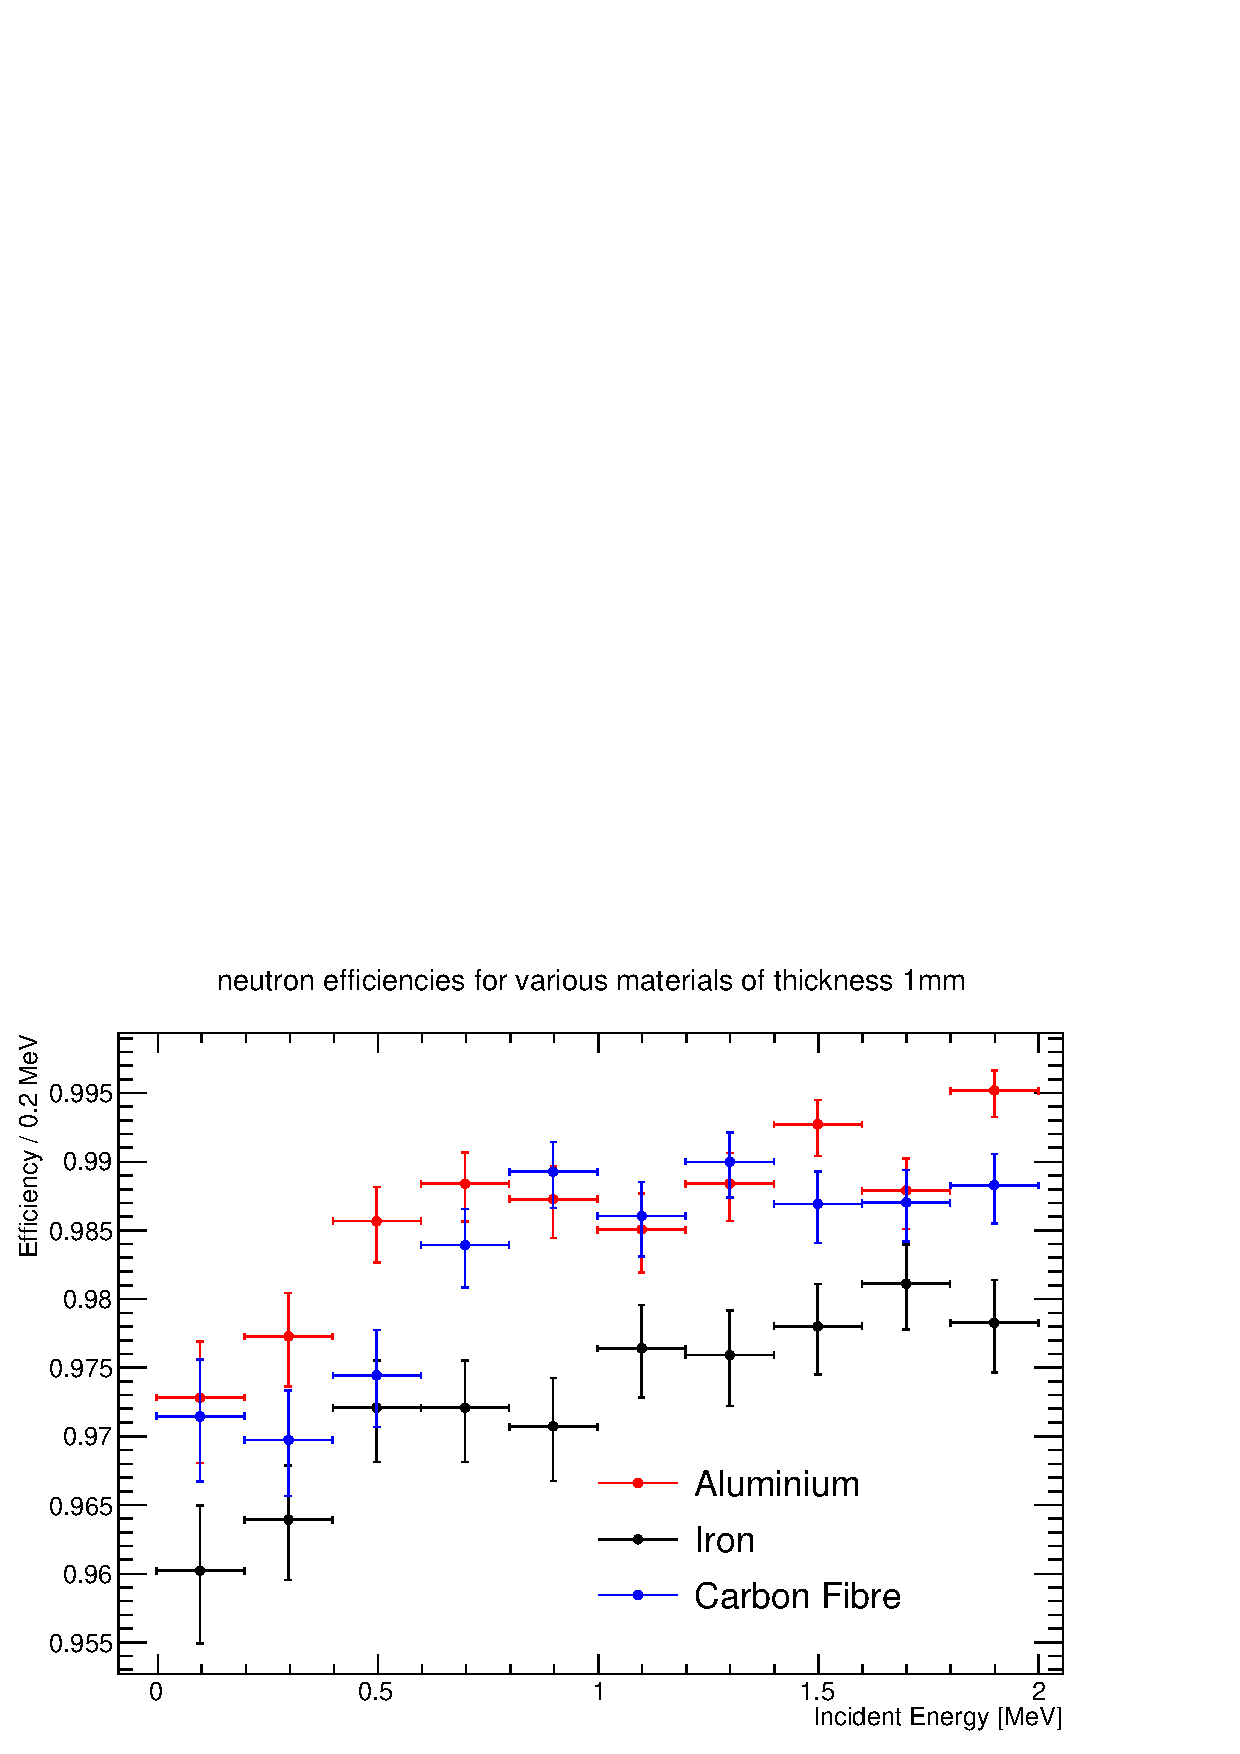
\includegraphics[width=75mm]{Chapter6/figures/neutron1mmMaterialsEfficiency0-2MeV.png}
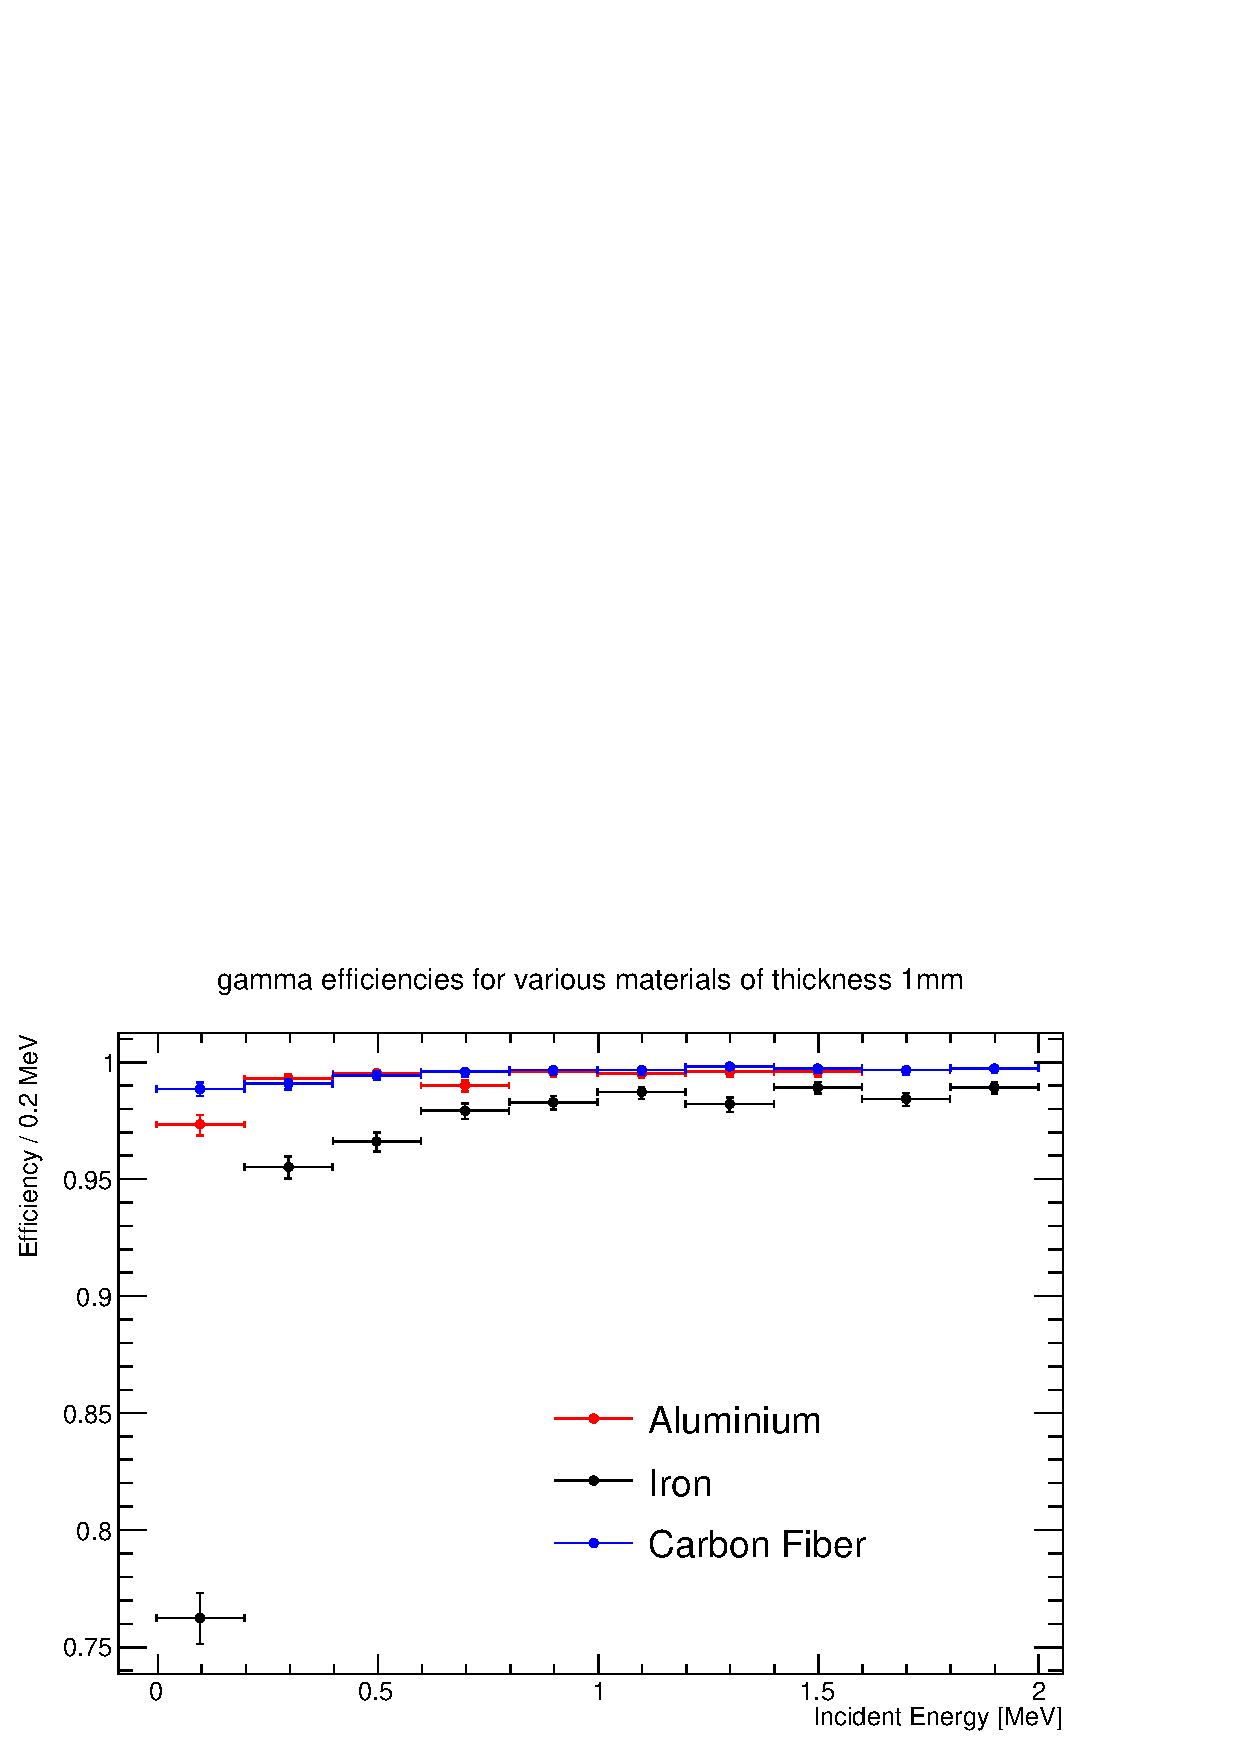
\includegraphics[width=75mm]{Chapter6/figures/gamma1mmMaterialsEfficiency0-2MeV.png}
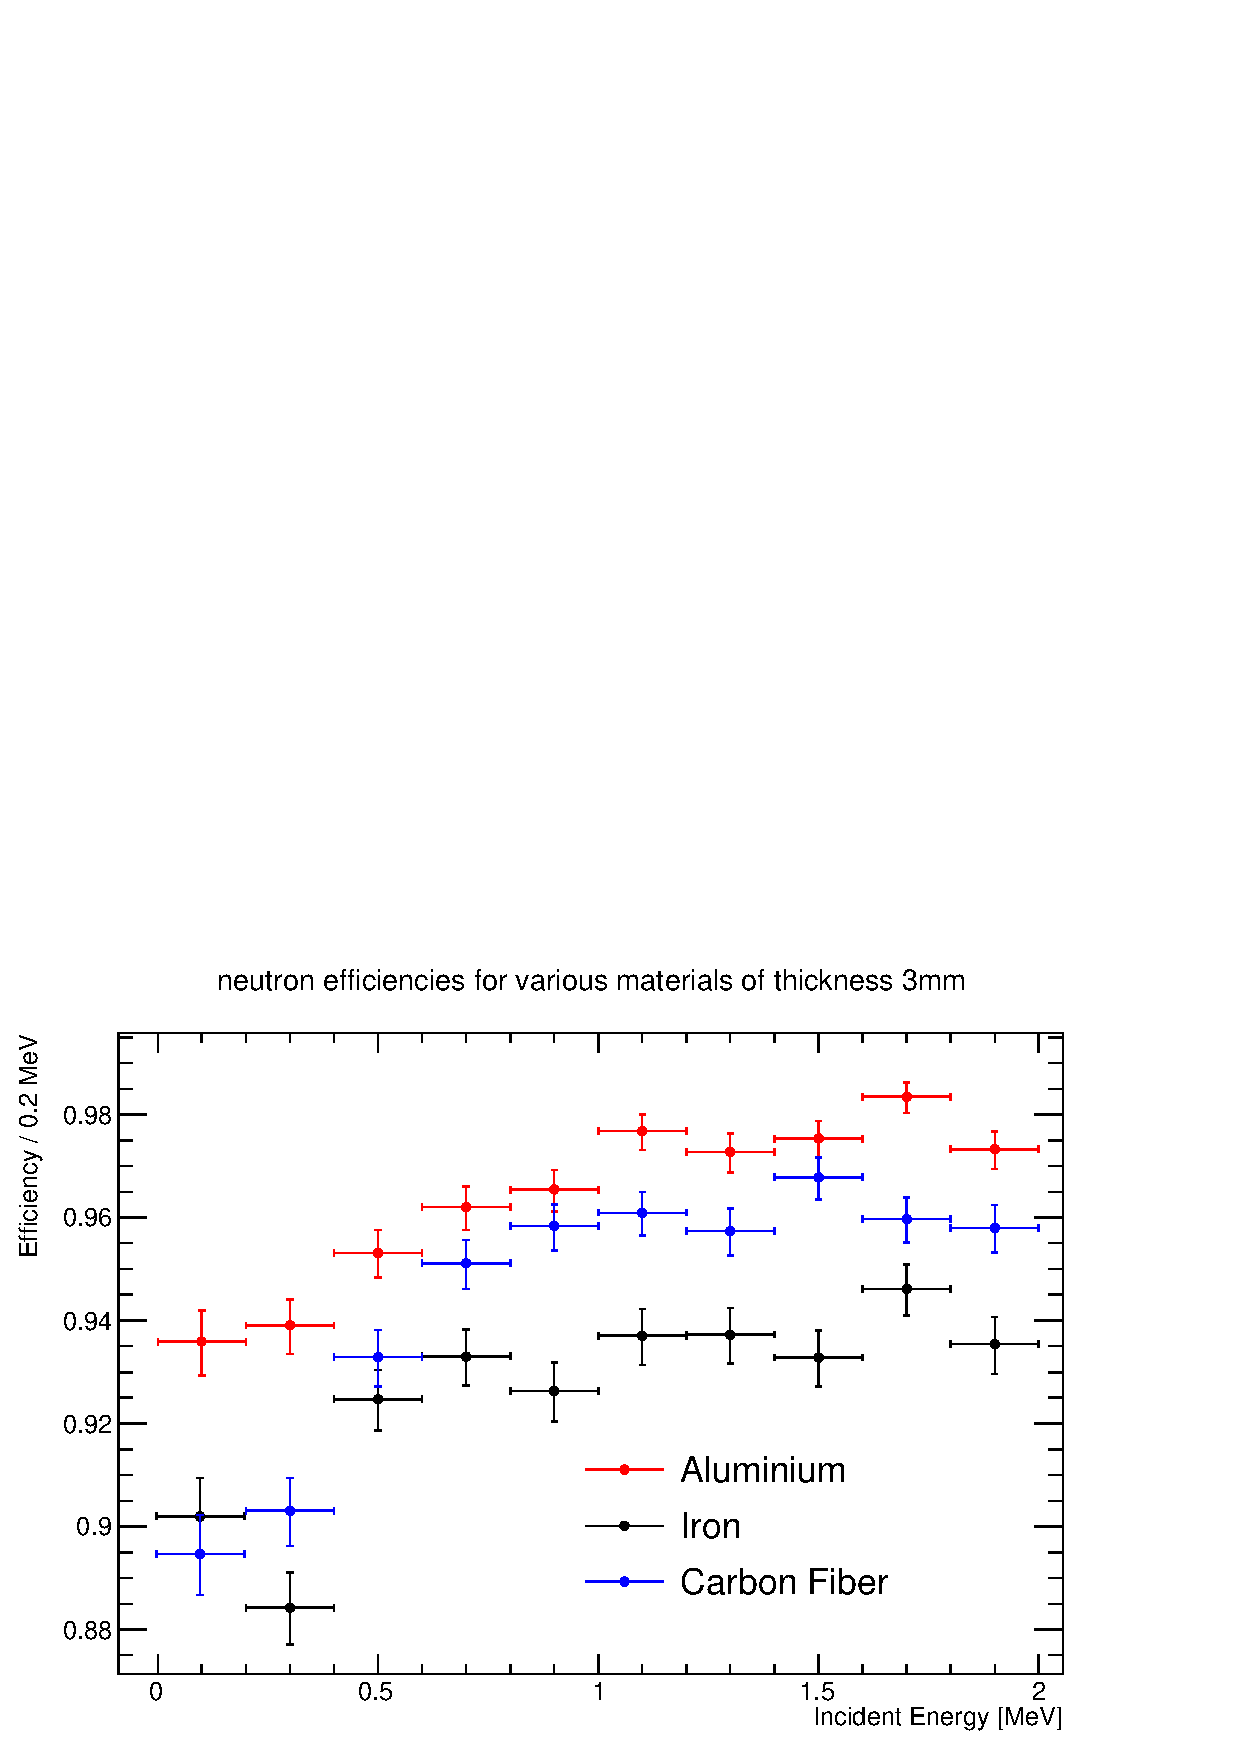
\includegraphics[width=75mm]{Chapter6/figures/neutron3mmMaterialsEfficiency0-2MeV.png}
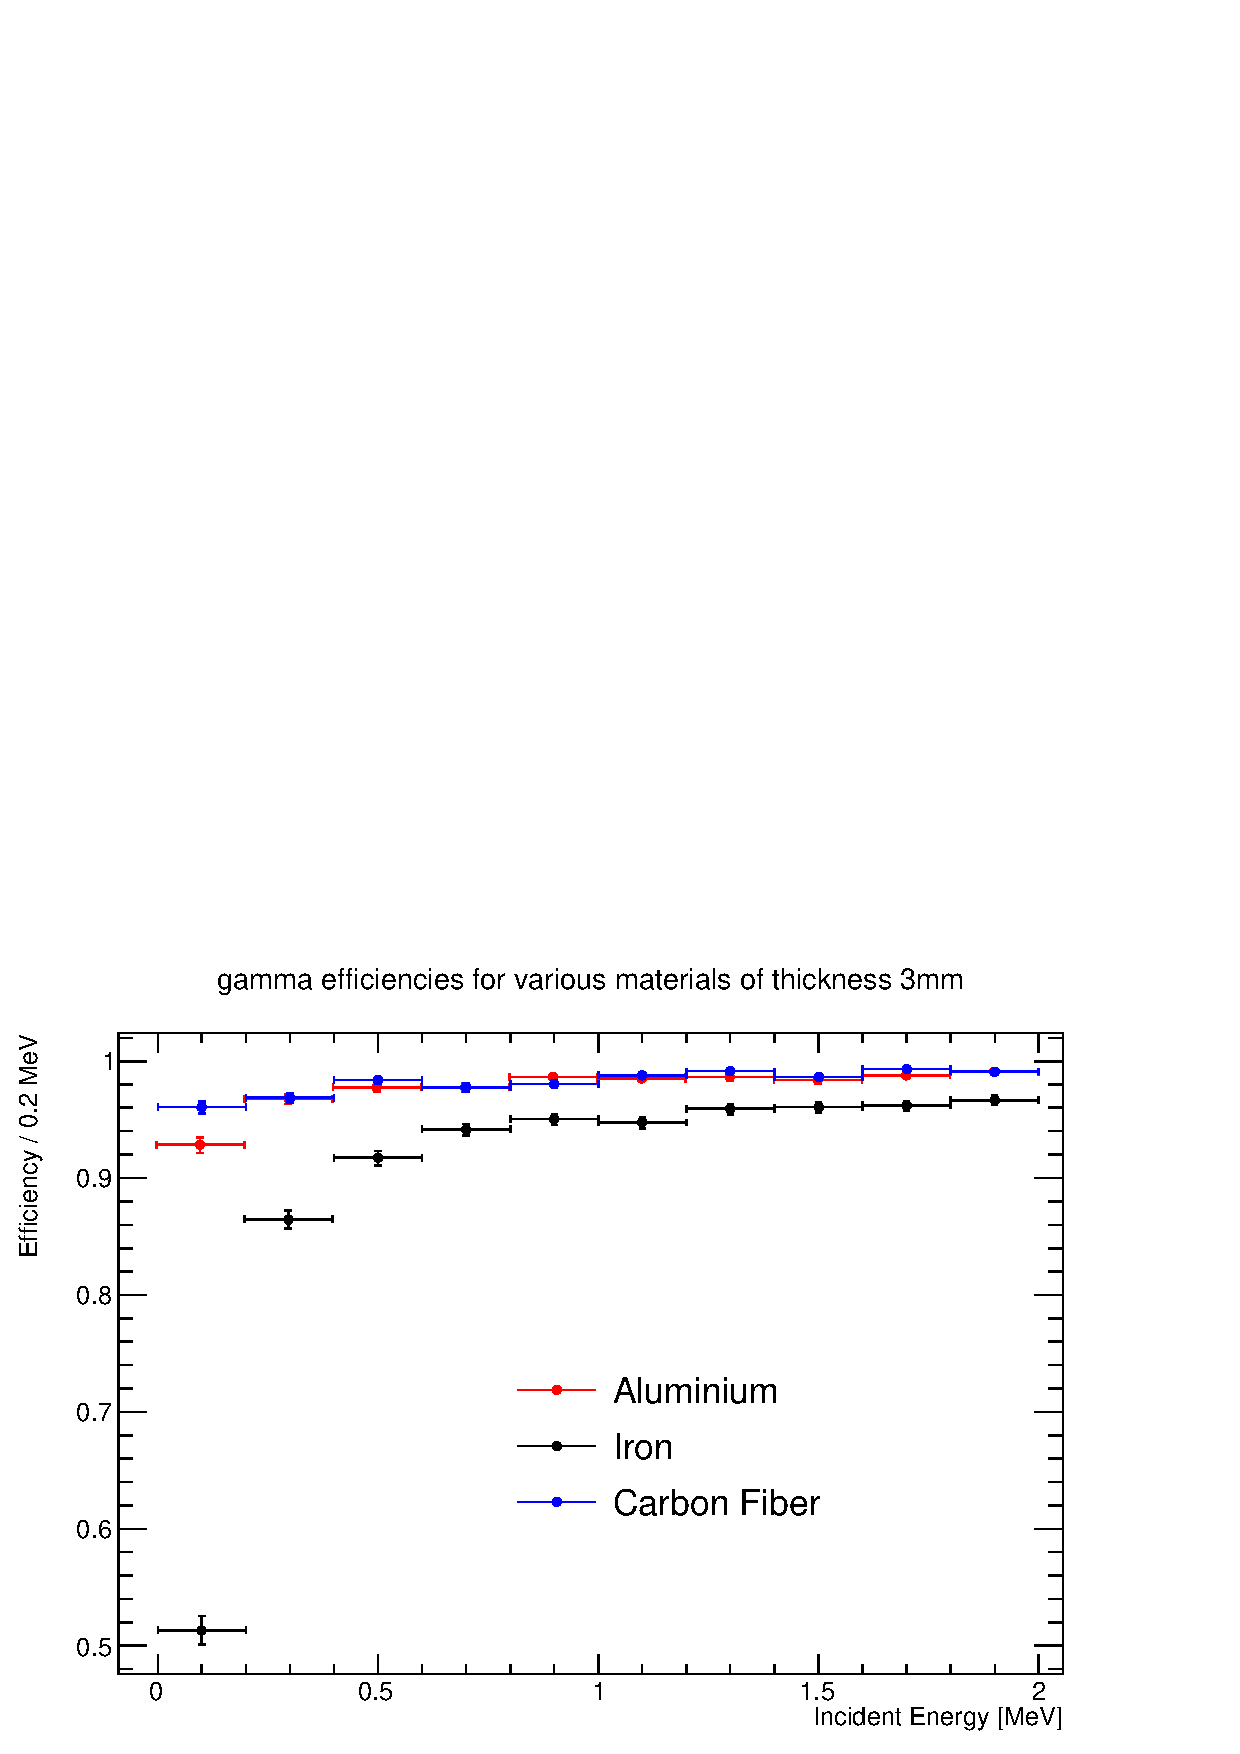
\includegraphics[width=75mm]{Chapter6/figures/gamma3mmMaterialsEfficiency0-2MeV.png}
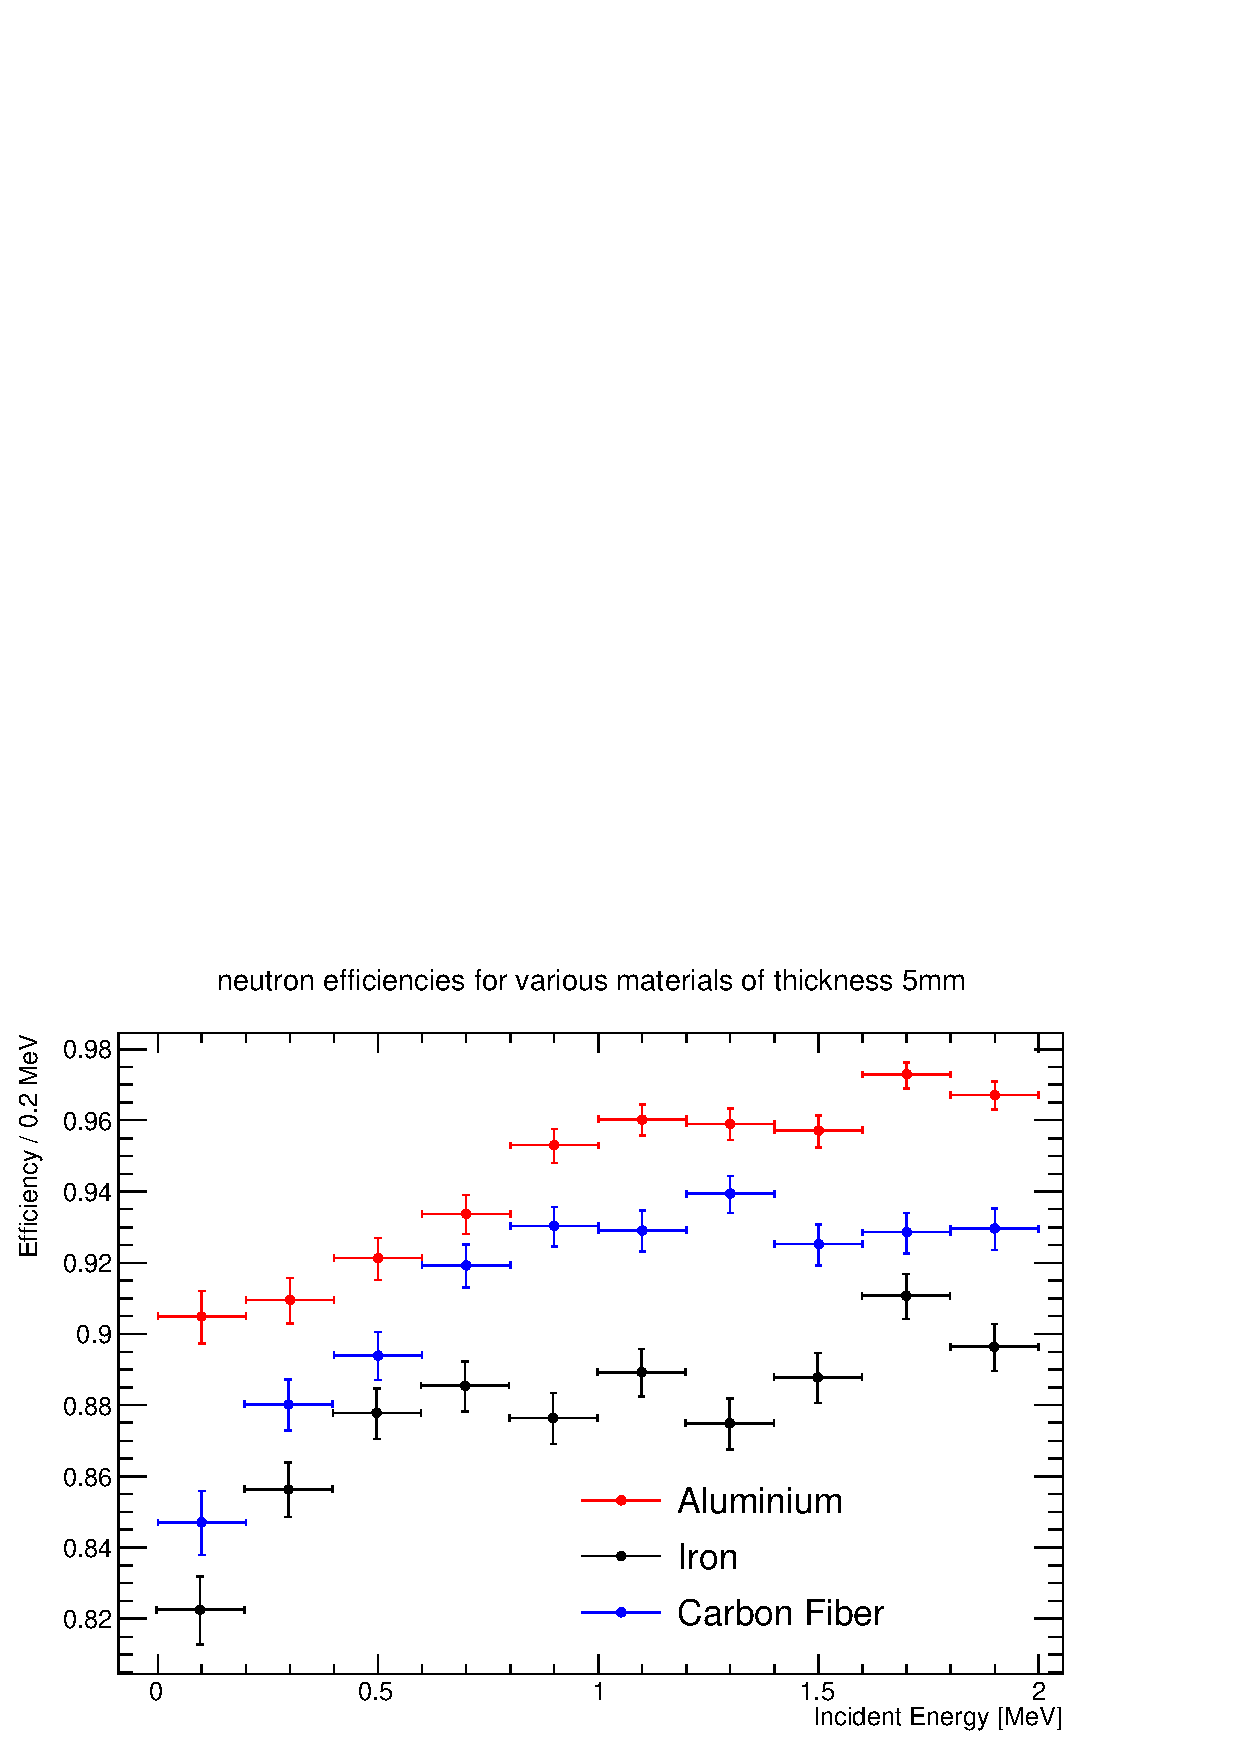
\includegraphics[width=75mm]{Chapter6/figures/neutron5mmMaterialsEfficiency0-2MeV.png}
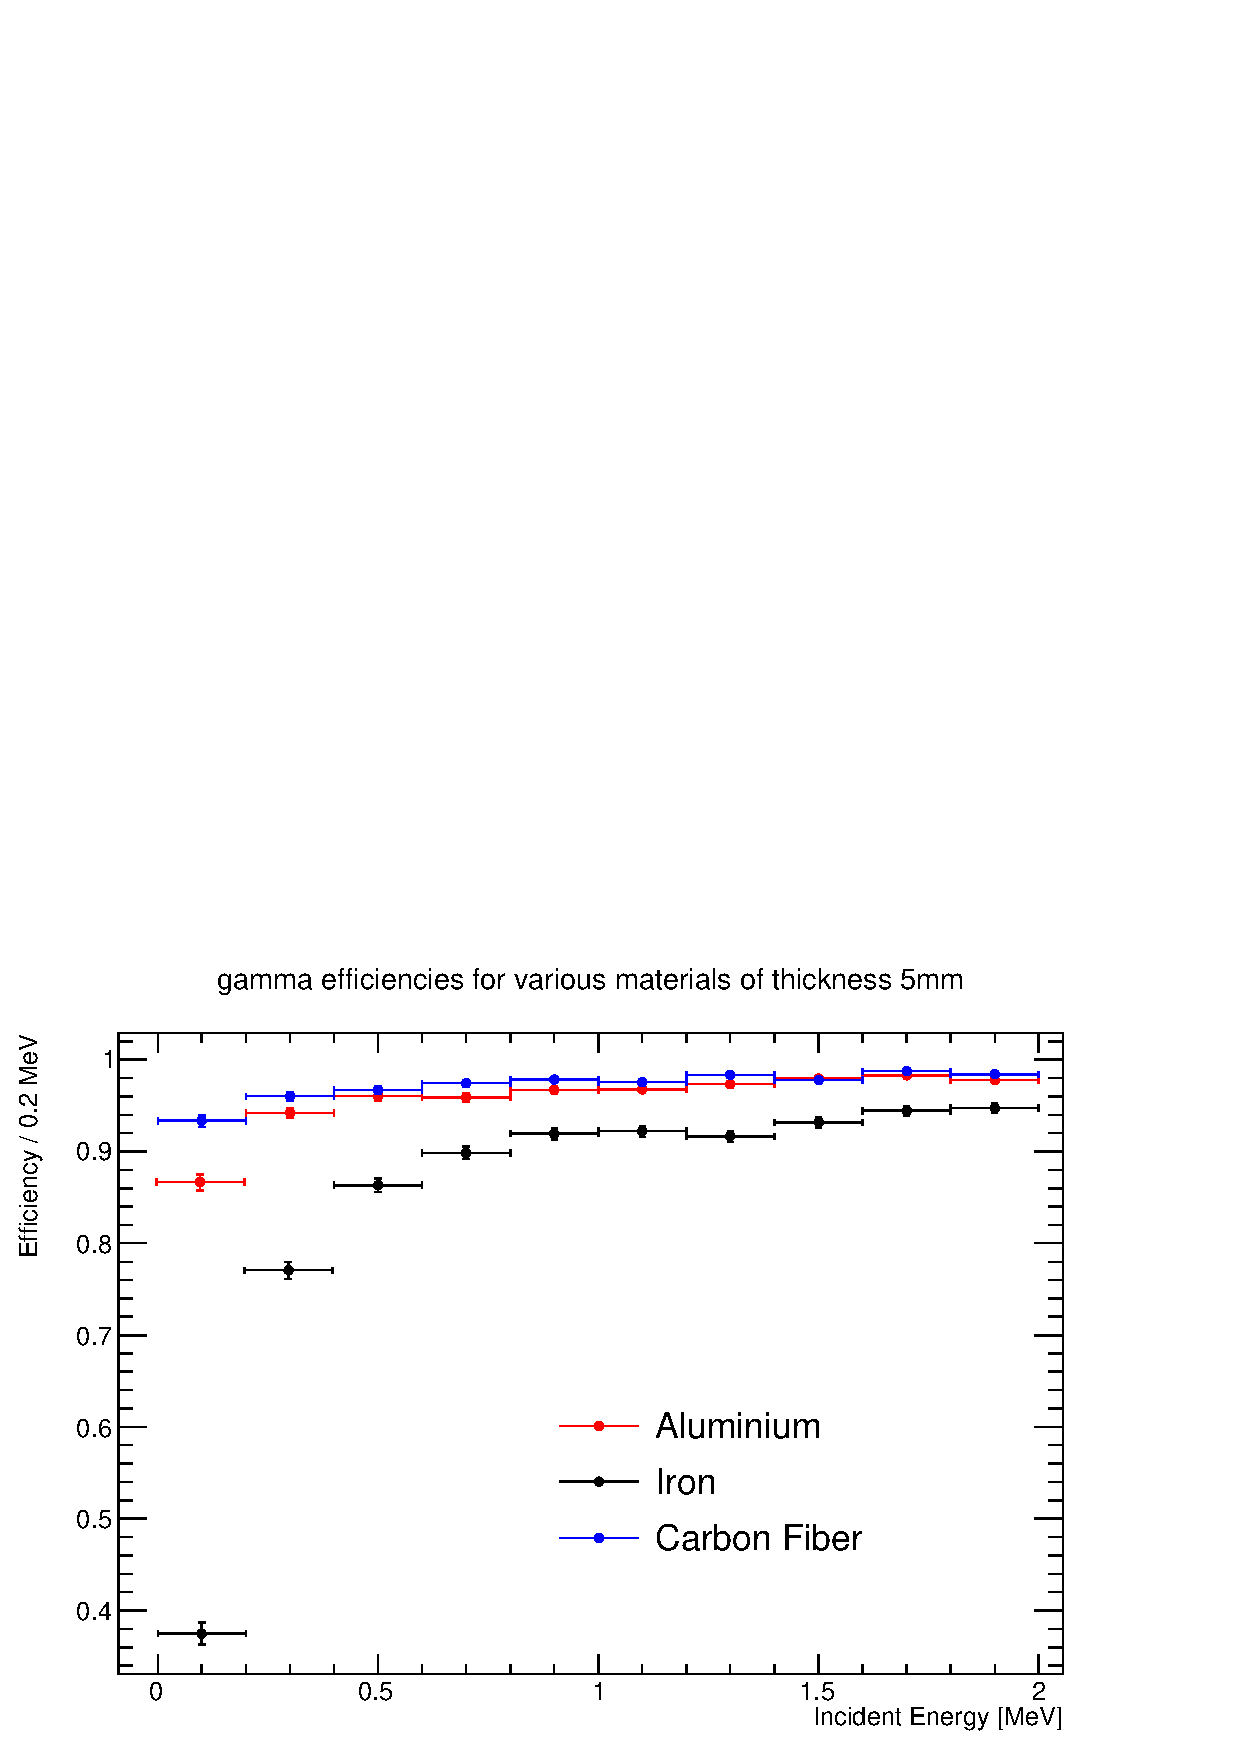
\includegraphics[width=75mm]{Chapter6/figures/gamma5mmMaterialsEfficiency0-2MeV.png}
\caption{The neutron (left) and gamma (right) efficiencies for carbon fibre, Iron and aluminium casings of 1 (top), 3 (middle) and 5 mm (bottom) thicknesses for lower energies between 0 and 2 MeV.}
\label{fig:efficienciesMaterialZoom}
\end{center}
\end{figure}
\newpage

Due to the Hydrogen atoms in the carbon fiber, the neutron efficiencies are not as great as aluminium at lower energies. Neutrons incident on hydrogen can transfer up to 100\% of their energy from one scatter alone, as opposed to aluminium at 14\% per scatter. This results in an increase in absorbed neutrons for carbon fiber. With a lower density than aluminium the efficiencies improve at higher energies however. At almost three times as dense as aluminium and four times as dense as carbon fibre, Iron is unsurprisingly much less efficient than the two.

\section{Electronics and Connection Design}
With the detectors in separate containers, the rest of the system can be localised into two separate boxes, one containing the FE, DAQ, HV-PS, IS and BMS, while the other is the battery used to provide power to the system. Figure \ref{fig:systemArchitecture} shows the system architecture.

\begin{figure}[htbp]
\begin{center}
\includegraphics[width=130mm]{Chapter6/figures/systemArchitecture.png}
\caption{The system architecture.}
\label{fig:systemArchitecture}
\end{center}
\end{figure}

\section{Container Construction}
The University of Liverpool were responsible for the design and production of the containers needed for the detectors, electronics and computer system. 
\subsection{Detector Containers}
The construction of the main body of the detector containers involves two C-shape panels bonded together with open ends for the detector installation. The end plates are made from a different material to the casing, 4.15 mm thick aluminium composite with a Polyethylene core. The material for the end plates is not of concern to the detection efficiency as they do not obstruct the detectors path of detection. The external connectors are fitted through one end of these plates, which are described later. The weight of each end is 0.2 kg for the neutron detector container and 0.24 kg for the gamma detector container, with each box requiring two, one for each end. The weight of the neutron and gamma containers are then 4.7 kg and 4.4 kg respectively. 

\begin{figure}[htbp]
\begin{center}
\includegraphics[width=100mm]{Chapter6/figures/detectorContainers.jpg}
\caption{The detector containers.}
\label{fig:detectorContainers}
\end{center}
\end{figure}

\subsection{The Neutron Detector Rack}
To support each pair of neutron detectors inside the containers requires a stable and secure structure. Aluminium is again used for the brackets to hold the detectors such that they do not obstruct the detection volume and are clamped on the external part of the PMT tube casing. A silicon resin is applied on the inside of the saddles to hold the detectors securely and after detector installation are fastened shut with screws. This can be seen in figure \ref{fig:neutronDetectorRackImages}. The whole support structure has a total weight of 0.542 kg and can be seen in figure \ref{fig:neutronDetectorRack}. In contrast there is no such structure needed for the gamma detectors and is simply fastened to the case via two raised aluminium and plastic blocks, shown in figure \ref{fig:gammaSupportStructure}.

\begin{figure}[htbp]
\begin{center}
\includegraphics[width=75mm]{Chapter6/figures/neutronDetectorRack1.png}
\includegraphics[width=75mm]{Chapter6/figures/neutronDetectorRack2.jpg}
\caption{The components of the neutron detector support structure. Left: The saddle clasp applied once detectors are installed. Right: The resin applied to the main structure just before inserting the detectors.}
\label{fig:neutronDetectorRackImages}
\end{center}
\end{figure}

\begin{figure}[htbp]
\begin{center}
\includegraphics[width=110mm]{Chapter6/figures/neutronDetectorRackGraphic.png}
\caption{The neutron detector support structure.}
\label{fig:neutronDetectorRack}
\end{center}
\end{figure}

\begin{figure}[htbp]
\begin{center}
\includegraphics[width=74mm]{Chapter6/figures/gammaSupport1.jpg}
\includegraphics[width=74mm]{Chapter6/figures/gammaSupport2.jpg}
\caption{The gamma detector support structure. Left: Side view. Right: Birds eye view.}
\label{fig:gammaSupportStructure}
\end{center}
\end{figure}

\subsection{The Electronics and Computer Equipment Container}
The housing for the electronics and the computer, along with all the corresponding equipment is made from the same aluminium composite used for the detector container ends. The box has dimensions 350 $\times$ 450 $\times$ 450 mm and is split into two compartments, shown in figure \ref{fig:electronicsBox}. The lower compartment is to be used for all cabling and the top compartment is then to be used for the HV-PS, FE, DAQ, BMS and the IS. The lower floor also acts to provide ventilation to the equipment above. Each face of the box is held with screws which are fastened to a box frame. Thus each panel can be removed easily and allows internal access if equipment is in need of repair or replacement. Two C-shaped plastic handles are attached on the top face to allow users to easily and safely carry the box.

\begin{figure}[htbp]
\begin{center}
\includegraphics[width=75mm]{Chapter6/figures/electronicsBox3.jpg}
\includegraphics[width=75mm]{Chapter6/figures/electronicsBox2.jpg}
\caption{Left: The container for the electronics and computer system. Right: The frame structure of the box.}
\label{fig:electronicsBox}
\end{center}
\end{figure}

The battery does not require a container as it is already encased in a protective casing. It has one single external connection, which is protected by thick plastic shielding to prevent users from electrocution and only the matching connector will complete the connection, shown in figure \ref{fig:battery}. The weight of the battery is 17.3 kg. 

\begin{figure}[htbp]
\begin{center}
\includegraphics[width=75mm]{Chapter6/figures/battery.jpg}
\caption{The battery connected with the correct cable.}
\label{fig:battery}
\end{center}
\end{figure}

\section{Integration}
With the exception of the detector and electronics containers, all of the equipment (detectors, computer, cables and connectors) was brought together and tested at Arktis Laboratories in Zurich. On completion of this, these parts were then shipped to the University of Liverpool for the integration phase of the prototype system.  

\subsection{Installation of the High Pressure Gas Detectors}
From the twelve detectors described only ten arrived at Liverpool, with one fast neutron and  one gamma detector missing from the inventory. Due to technical issues they were tested independently, then subsequently shipped and installed after the integration at Liverpool.

Each neutron tube is inserted in the detector rack with the resin applied to each clasp and then fixed shut with screws and a bolt fasten, shown in figure \ref{fig:neutronDetClasp}. A plastic angular holder, shown in figure \ref{fig:neutronDetHolder}, is used to hold them parallel to each other and avoid slipping inside the container. The tubes are then slid into the containers via the open ends and fastened with screws, this can be seen in figure \ref{fig:neutronDetInstalled}. The cables for the PMT's and the readout are then tied neatly and fed to one end of the box. To enable external connection with each container an end plate is fixed to the boxes which provides such an interface, shown left in figure \ref{fig:neutronBoxEnd}. The cables are matched with numerical labels and each end is fixed with screws. A plastic C-shaped handle is placed on each end of the box to enable the user to lift the box, shown in figure \ref{fig:neutronBoxEnd}. The total weight of the neutron box upon installation is then 18.6 kg, well below the 25 kg limit imposed. 

\begin{figure}[htbp]
\begin{center}
\includegraphics[width=75mm]{Chapter6/figures/neutronTubeFixing1.jpg}
\caption{The neutron detectors fixed inside the rack with the clasp fixed.}
\label{fig:neutronDetClasp}
\end{center}
\end{figure}

\begin{figure}[htbp]
\begin{center}
\includegraphics[width=75mm]{Chapter6/figures/neutronTubeHolder1.jpg}
\caption{The plastic piece used to hold the detectors parallel and securely inside the box.}
\label{fig:neutronDetHolder}
\end{center}
\end{figure}

\begin{figure}[htbp]
\begin{center}
\includegraphics[width=75mm]{Chapter6/figures/neutronTubes1.jpg}
\caption{The neutron detectors ready for insertion in the containers.}
\label{fig:neutronDetTubes}
\end{center}
\end{figure}

\begin{figure}[htbp]
\begin{center}
\includegraphics[width=74mm]{Chapter6/figures/neutronTubesInstall1.jpg}
\includegraphics[width=74mm]{Chapter6/figures/neutronTubesInstall2.jpg}
\caption{The neutron detectors installed in the containers.}
\label{fig:neutronDetInstalled}
\end{center}
\end{figure}

\begin{figure}[htbp]
\begin{center}
\includegraphics[width=74mm]{Chapter6/figures/neutronContainerEnd1.jpg}
\includegraphics[width=74mm]{Chapter6/figures/neutronContainerEnd2.jpg}
\caption{The neutron detector container ends. Left: Cable connection side. Right: Blank side.}
\label{fig:neutronBoxEnd}
\end{center}
\end{figure}

For the gamma detector, the support structure is fixed to the container base with screws and bolts. The detector is then placed on these fixings and fastened with an aluminium clasp, this can be seen in figure \ref{fig:gammaDetClasp}. A thin compressible pad (1 cm thick) is inserted between the detector and the container base to provide shock relief, as the detector may come into contact with the container base. 
An additional feature on the gamma containers is a small coin shaped slot on the side facing the detector allowing calibration sources to be placed inside the container, right in figure \ref{fig:gammaDetClasp}. Also a similar entry point is inserted on the end of the container to allow placement of sources internally via a rod, this is covered with a plastic cap and is shown in figure \ref{fig:gammaBoxEnd}. The fully installed gamma box has a total weight of 17.5 kg.

\begin{figure}[htbp]
\begin{center}
\includegraphics[width=74mm]{Chapter6/figures/gammaDetClasp1.jpg}
\includegraphics[width=74mm]{Chapter6/figures/gammaDetSlot1.jpg}
\caption{Left: The gamma detector fixed with the clasp, ready for installation in the box.
Right: A coin shaped slot on gamma detector container with a retractable plastic piece to hold a small calibration source.}
\label{fig:gammaDetClasp}
\end{center}
\end{figure}

\begin{figure}[htbp]
\begin{center}\includegraphics[width=100mm]{Chapter6/figures/gammaContainerEnd2.jpg}
\caption{The gamma detector container end with the entry point for sources.}
\label{fig:gammaBoxEnd}
\end{center}
\end{figure}

Temperature and pressure sensors were added separately after installation of the detectors. These were omitted from the Liverpool integration and fitted inside the containers at a facility in Poland prior to preliminary tests of the system.

\subsection{Installation of the Electronics and Computer}
The electronics system cabling can be summarised by figure \ref{fig:electronicsDiagram}. It contains three HV-PS modules, each with four output connections and three 14-bit 500 MS/s FE modules (labelled as digitizer), each with 8 input connections. With two PMT's per detector four cables into the FE are required for each neutron box and two for the gamma box. Only one high voltage cable is required for each detector. An optical connection from FE + HV-PS unit to the PC is established via the DAQ (labelled as A3818). This is mounted inside the PC through the x8/x16 PCI Express slot and can solely handle all 6 of the front end modules. The HV-PS, FE and DAQ are all produced by CAEN but the modules used were developed for bespoke use in the MODES-SNM project, all shown in figure \ref{fig:caenModules}. 

\begin{figure}[htbp]
\begin{center}
\includegraphics[width=90mm]{Chapter6/figures/electronicsSetupDiagram.png}
\caption{The overview of the internal cabling required for the HV-PS, FE, DAQ, BMS and the IS.}
\label{fig:electronicsDiagram}
\end{center}
\end{figure}

\begin{figure}[htbp]
\begin{center}
\includegraphics[width=74mm]{Chapter6/figures/caenHV-PS.png}
\includegraphics[width=74mm]{Chapter6/figures/caenDigitizer.png} \\
\includegraphics[width=74mm]{Chapter6/figures/caenDAQ.png}
\caption{From top left clockwise: The HV-PS, FE and DAQ produced and developed by CAEN.}
\label{fig:caenModules}
\end{center}
\end{figure}

The BMS, GPS and Slow Control (SC - labelled RS485) all follow USB protocol connection to the core of the IS, the PC. The SC is used to control the gas pressure, temperature and PMT voltages for each detector, while the BMS monitors and regulates the current and voltage supplied from the battery to the system. 

The computer and components all require 12 V input which is supplied from the battery. An external mechanical switch is required outside the container to control this power supply. Wired in series with the PC and the Power Distribution (PD) the battery can then be disconnected from the system, acting as a kill switch, using a key which is shown left in figure \ref{fig:powerSwitchAndDistribution}. The PD consists of a series of conducting connectors in order to provide voltage across the WiFi router, FE and HV-PS, right in figure \ref{fig:powerSwitchAndDistribution}.

\begin{figure}[htbp]
\begin{center}
\includegraphics[width=74mm]{Chapter6/figures/powerSwitch.jpg}
\includegraphics[width=74mm]{Chapter6/figures/powerDistribution.jpg}
\caption{Left: The external mechanical switch located on the electronics container. Right: The power distribution used to supply 12 V to the HV-PS, FE and WiFi router fully wired up.}
\label{fig:powerSwitchAndDistribution}
\end{center}
\end{figure}

The three HV-PS and three digitisers are stacked upon each other and are secured via four aluminium pillars on each corner of the module tower. Each is fastened to the containers raised floor with the top joined by two parallel metal bars. There is a $\sim$1 cm gap between each layer due to small rubber feet under each component, providing stability. This structure design does not impede on the component fans, which are located on the side of each component, and allows plenty of ventilation. The PC unit is fastened to the same floor in the container using existing holes in the factory casing of the PC. The WiFi router is then fastened on top of this. 

Although most components have built-in fans, additional ventilation is required for the container itself to dissipate heat from cabling and the components inside the container. The total system in operation draws $\sim$21 A of current, this is a considerable power consumption of $\sim$250 W. Fans are implemented to maintain room temperature inside the box, although the system can operate in temperatures varying 0 - 45 \textdegree C. Considering the increase in power consumption from the addition of fans and the surface area restrictions on the box, four small 0.25 mA fans are used. Mounting these on two opposite container sides, one near the top and one near the bottom, repeated on the opposite face, provides adequate cooling. The two on the bottom provide external air into the box with the top two operated in reverse expelling warmer air to the outside of the box. This was tested with the temperature monitored every 30 mins for a 3 hour continuous run. The temperature increased by 4 \textdegree C above room temperature at the end of the running period, but this level was reached within an hour and an increase of 2.5 \textdegree C after just 30 minutes. This is a perfectly acceptable level of temperature increase as the system remained fully operational throughout and considering that the battery can last no longer than 8 hours is a very reasonable testing time.

To allow external connection to the components, panels are removed from two opposite sides of the container to facilitate this. To make the electronics and computer easily accessible incase of a component failure or a wiring fault, it is necessary to restrict all external connections to only 2 of the 4 side faces. Seven holes are required for the detectors, four for the fans, one for the key, one for the battery, one for the mains supply, one for the antenna and then five for various USB, ethernet and VGA connections. This can be seen in figure \ref{fig:electronicsBoxSides}. Harting connectors are used as the external cables to connect each module. These are shown in figure \ref{fig:hartingCables}.

\begin{figure}[htbp]
\begin{center}
\includegraphics[width=74mm]{Chapter6/figures/electronicsBoxSide1.jpg} 
\includegraphics[width=74mm]{Chapter6/figures/electronicsBoxSide2.jpg} 
\caption{The left and right sides of the electronics box with the full fittings and connectors mounted.}
\label{fig:electronicsBoxSides}
\end{center}
\end{figure}

\begin{figure}[htbp]
\begin{center}
\includegraphics[width=74mm]{Chapter6/figures/hartingCables1.jpg} 
\includegraphics[width=60mm]{Chapter6/figures/hartingCables3.png} 
\caption{Left: The Harting cables connected to the electronics box. Right: The front end view of the Harting connectors.}
\label{fig:hartingCables}
\end{center}
\end{figure}

The fully integrated electronics and computer system can be seen installed in the container with all cabling in figure \ref{fig:electronicsBoxInstalledOpen}. With the inclusion of two handles on top of the container the total weight of the closed electronics box is 32.7 kg. This weight exceeds the limit of 25 kg imposed on each module but this restriction is relaxed for the electronics box as it is preferable to have one single module for the electronics. A large contribution of the total weight is due to the detector connectors, as each weighs $\sim$2 kg. This was unforeseen in the design but is acceptable for a prototype model.

\begin{figure}[htbp]
\begin{center}
\includegraphics[width=100mm]{Chapter6/figures/electronicsBoxInstalledOpenAnnotated.jpg}
\caption{The fully installed electronics and computer system cabled in the container with the two front and back panels removed.}
\label{fig:electronicsBoxInstalledOpen}
\end{center}
\end{figure}

The total weight of the whole MODES-SNM prototype is then close to 185 kg. This however omits the weight of the Harting cables. The full prototype can be seen in figure \ref{fig:fullSystem}.

\begin{figure}[htbp]
\begin{center}
\includegraphics[width=80mm]{Chapter6/figures/fullSystem2.jpg}
\caption{The full system prototype.}
\label{fig:fullSystem}
\end{center}
\end{figure}

